% Options for packages loaded elsewhere
\PassOptionsToPackage{unicode}{hyperref}
\PassOptionsToPackage{hyphens}{url}
%
\documentclass[
  12pt,
  a4paper,
  onecolumn, twoside]{article}
\usepackage{amsmath,amssymb}
\usepackage{lmodern}
\usepackage{setspace}
\usepackage{iftex}
\ifPDFTeX
  \usepackage[T1]{fontenc}
  \usepackage[utf8]{inputenc}
  \usepackage{textcomp} % provide euro and other symbols
\else % if luatex or xetex
  \usepackage{unicode-math}
  \defaultfontfeatures{Scale=MatchLowercase}
  \defaultfontfeatures[\rmfamily]{Ligatures=TeX,Scale=1}
  \setmainfont[]{Times New Roman}
\fi
% Use upquote if available, for straight quotes in verbatim environments
\IfFileExists{upquote.sty}{\usepackage{upquote}}{}
\IfFileExists{microtype.sty}{% use microtype if available
  \usepackage[]{microtype}
  \UseMicrotypeSet[protrusion]{basicmath} % disable protrusion for tt fonts
}{}
\makeatletter
\@ifundefined{KOMAClassName}{% if non-KOMA class
  \IfFileExists{parskip.sty}{%
    \usepackage{parskip}
  }{% else
    \setlength{\parindent}{0pt}
    \setlength{\parskip}{6pt plus 2pt minus 1pt}}
}{% if KOMA class
  \KOMAoptions{parskip=half}}
\makeatother
\usepackage{xcolor}
\usepackage[left=3cm, right=2cm, top=2cm, bottom=3cm]{geometry}
\usepackage{color}
\usepackage{fancyvrb}
\newcommand{\VerbBar}{|}
\newcommand{\VERB}{\Verb[commandchars=\\\{\}]}
\DefineVerbatimEnvironment{Highlighting}{Verbatim}{commandchars=\\\{\}}
% Add ',fontsize=\small' for more characters per line
\usepackage{framed}
\definecolor{shadecolor}{RGB}{248,248,248}
\newenvironment{Shaded}{\begin{snugshade}}{\end{snugshade}}
\newcommand{\AlertTok}[1]{\textcolor[rgb]{0.94,0.16,0.16}{#1}}
\newcommand{\AnnotationTok}[1]{\textcolor[rgb]{0.56,0.35,0.01}{\textbf{\textit{#1}}}}
\newcommand{\AttributeTok}[1]{\textcolor[rgb]{0.77,0.63,0.00}{#1}}
\newcommand{\BaseNTok}[1]{\textcolor[rgb]{0.00,0.00,0.81}{#1}}
\newcommand{\BuiltInTok}[1]{#1}
\newcommand{\CharTok}[1]{\textcolor[rgb]{0.31,0.60,0.02}{#1}}
\newcommand{\CommentTok}[1]{\textcolor[rgb]{0.56,0.35,0.01}{\textit{#1}}}
\newcommand{\CommentVarTok}[1]{\textcolor[rgb]{0.56,0.35,0.01}{\textbf{\textit{#1}}}}
\newcommand{\ConstantTok}[1]{\textcolor[rgb]{0.00,0.00,0.00}{#1}}
\newcommand{\ControlFlowTok}[1]{\textcolor[rgb]{0.13,0.29,0.53}{\textbf{#1}}}
\newcommand{\DataTypeTok}[1]{\textcolor[rgb]{0.13,0.29,0.53}{#1}}
\newcommand{\DecValTok}[1]{\textcolor[rgb]{0.00,0.00,0.81}{#1}}
\newcommand{\DocumentationTok}[1]{\textcolor[rgb]{0.56,0.35,0.01}{\textbf{\textit{#1}}}}
\newcommand{\ErrorTok}[1]{\textcolor[rgb]{0.64,0.00,0.00}{\textbf{#1}}}
\newcommand{\ExtensionTok}[1]{#1}
\newcommand{\FloatTok}[1]{\textcolor[rgb]{0.00,0.00,0.81}{#1}}
\newcommand{\FunctionTok}[1]{\textcolor[rgb]{0.00,0.00,0.00}{#1}}
\newcommand{\ImportTok}[1]{#1}
\newcommand{\InformationTok}[1]{\textcolor[rgb]{0.56,0.35,0.01}{\textbf{\textit{#1}}}}
\newcommand{\KeywordTok}[1]{\textcolor[rgb]{0.13,0.29,0.53}{\textbf{#1}}}
\newcommand{\NormalTok}[1]{#1}
\newcommand{\OperatorTok}[1]{\textcolor[rgb]{0.81,0.36,0.00}{\textbf{#1}}}
\newcommand{\OtherTok}[1]{\textcolor[rgb]{0.56,0.35,0.01}{#1}}
\newcommand{\PreprocessorTok}[1]{\textcolor[rgb]{0.56,0.35,0.01}{\textit{#1}}}
\newcommand{\RegionMarkerTok}[1]{#1}
\newcommand{\SpecialCharTok}[1]{\textcolor[rgb]{0.00,0.00,0.00}{#1}}
\newcommand{\SpecialStringTok}[1]{\textcolor[rgb]{0.31,0.60,0.02}{#1}}
\newcommand{\StringTok}[1]{\textcolor[rgb]{0.31,0.60,0.02}{#1}}
\newcommand{\VariableTok}[1]{\textcolor[rgb]{0.00,0.00,0.00}{#1}}
\newcommand{\VerbatimStringTok}[1]{\textcolor[rgb]{0.31,0.60,0.02}{#1}}
\newcommand{\WarningTok}[1]{\textcolor[rgb]{0.56,0.35,0.01}{\textbf{\textit{#1}}}}
\usepackage{longtable,booktabs,array}
\usepackage{calc} % for calculating minipage widths
% Correct order of tables after \paragraph or \subparagraph
\usepackage{etoolbox}
\makeatletter
\patchcmd\longtable{\par}{\if@noskipsec\mbox{}\fi\par}{}{}
\makeatother
% Allow footnotes in longtable head/foot
\IfFileExists{footnotehyper.sty}{\usepackage{footnotehyper}}{\usepackage{footnote}}
\makesavenoteenv{longtable}
\usepackage{graphicx}
\makeatletter
\def\maxwidth{\ifdim\Gin@nat@width>\linewidth\linewidth\else\Gin@nat@width\fi}
\def\maxheight{\ifdim\Gin@nat@height>\textheight\textheight\else\Gin@nat@height\fi}
\makeatother
% Scale images if necessary, so that they will not overflow the page
% margins by default, and it is still possible to overwrite the defaults
% using explicit options in \includegraphics[width, height, ...]{}
\setkeys{Gin}{width=\maxwidth,height=\maxheight,keepaspectratio}
% Set default figure placement to htbp
\makeatletter
\def\fps@figure{htbp}
\makeatother
\setlength{\emergencystretch}{3em} % prevent overfull lines
\providecommand{\tightlist}{%
  \setlength{\itemsep}{0pt}\setlength{\parskip}{0pt}}
\setcounter{secnumdepth}{5}
\newlength{\cslhangindent}
\setlength{\cslhangindent}{1.5em}
\newlength{\csllabelwidth}
\setlength{\csllabelwidth}{3em}
\newlength{\cslentryspacingunit} % times entry-spacing
\setlength{\cslentryspacingunit}{\parskip}
\newenvironment{CSLReferences}[2] % #1 hanging-ident, #2 entry spacing
 {% don't indent paragraphs
  \setlength{\parindent}{0pt}
  % turn on hanging indent if param 1 is 1
  \ifodd #1
  \let\oldpar\par
  \def\par{\hangindent=\cslhangindent\oldpar}
  \fi
  % set entry spacing
  \setlength{\parskip}{#2\cslentryspacingunit}
 }%
 {}
\usepackage{calc}
\newcommand{\CSLBlock}[1]{#1\hfill\break}
\newcommand{\CSLLeftMargin}[1]{\parbox[t]{\csllabelwidth}{#1}}
\newcommand{\CSLRightInline}[1]{\parbox[t]{\linewidth - \csllabelwidth}{#1}\break}
\newcommand{\CSLIndent}[1]{\hspace{\cslhangindent}#1}
\ifLuaTeX
\usepackage[bidi=basic]{babel}
\else
\usepackage[bidi=default]{babel}
\fi
\babelprovide[main,import]{estonian}
% get rid of language-specific shorthands (see #6817):
\let\LanguageShortHands\languageshorthands
\def\languageshorthands#1{}
\usepackage{booktabs}
\usepackage{fvextra} % needed for code wrapping
\DefineVerbatimEnvironment{Highlighting}{Verbatim}{breaklines,commandchars=\\\{\}}
\usepackage{cancel}
\usepackage[version=4]{mhchem}
\usepackage{siunitx}
\usepackage{booktabs}
\usepackage{longtable}
\usepackage{array}
\usepackage{multirow}
\usepackage{wrapfig}
\usepackage{float}
\usepackage{colortbl}
\usepackage{pdflscape}
\usepackage{tabu}
\usepackage{threeparttable}
\usepackage{threeparttablex}
\usepackage[normalem]{ulem}
\usepackage{makecell}
\usepackage{xcolor}
\ifLuaTeX
  \usepackage{selnolig}  % disable illegal ligatures
\fi
\IfFileExists{bookmark.sty}{\usepackage{bookmark}}{\usepackage{hyperref}}
\IfFileExists{xurl.sty}{\usepackage{xurl}}{} % add URL line breaks if available
\urlstyle{same} % disable monospaced font for URLs
\hypersetup{
  pdftitle={Õhuniiskuse karakteristikute määramine},
  pdfauthor={peacecop kalmer:},
  pdflang={et},
  hidelinks,
  pdfcreator={LaTeX via pandoc}}

\title{Õhuniiskuse karakteristikute määramine}
\usepackage{etoolbox}
\makeatletter
\providecommand{\subtitle}[1]{% add subtitle to \maketitle
  \apptocmd{\@title}{\par {\large #1 \par}}{}{}
}
\makeatother
\subtitle{Viies laboratoorne töö soojusõpetuses}
\author{peacecop kalmer:}
\date{2022-07-01}

% \usepackage{fvextra} % needed for code wrapping

\begin{document}
\maketitle

{
\setcounter{tocdepth}{2}
\tableofcontents
}
\listoffigures
\listoftables
\setstretch{1.5}
\sisetup{inter-unit-product = \ensuremath { { } \times { } } }

\hypertarget{eesmuxe4rgid}{%
\section{Eesmärgid}\label{eesmuxe4rgid}}

\begin{enumerate}
\def\labelenumi{\arabic{enumi}.}
\item
  Õhuniiskuse peamiste karakteristikute ja vahenditega nende määramiseks tutvutud.
\item
  Õhu relatiivne ja absoluutne niiskus ning kastepunkt erinevate meetoditega katseliselt määratud.
\end{enumerate}

\hypertarget{vahendid}{%
\section{Vahendid}\label{vahendid}}

\begin{enumerate}
\def\labelenumi{\arabic{enumi}.}
\item
  anspiratsioonpsühhopeeter,
\item
  statsionaarne pühhomeeter,
\item
  läikiva välispinnag ametallist õõneskera statiivil,
\item
  temperatuurisensor,
\item
  jäätükid,
\item
  puhas riidelapp,
\item
  aknapuhastuse vahend,
\item
  destilleeritud vesi,
\item
  limasensor,
\item
  mitmeotstarbeline arvuti.
\end{enumerate}

\hypertarget{reeglid}{%
\section{Reeglid}\label{reeglid}}

\hypertarget{juxf5ud}{%
\subsection{Jõud}\label{juxf5ud}}

\begin{align}
\vec{F} := m \cdot \vec{a},
\label{eq:force}
\end{align}

kus \emph{m} on mass ja \emph{a} on kiirendus (\protect\hyperlink{ref-haynes_2014_crc}{Haynes 2014}, p.~2-2). Dimensionaalanalüüs:

\begin{align}
\mathrm{M \cdot \frac{L}{T^2} = \frac{L \cdot M}{T^2}},
\label{eq:dimensional-analysis-for-force}
\end{align}

mistõttu ühik on \(\unit{\meter\kilogram\per\second\squared}\) või lühemalt \(\unit{\newton}\).

\hypertarget{temperatuur}{%
\subsection{Temperatuur}\label{temperatuur}}

\begin{align}
T := t + 237.15,
\label{eq:absolute-temperature}
\end{align}

mille ühik on \(\unit{\kelvin}\) (\protect\hyperlink{ref-American_Society_of_Heating_Refrigerating_and_Air-Conditioning_Engineers2017-im}{American Society of Heating, Refrigerating and Air-Conditioning Engineers 2017}, p.~8).

\hypertarget{energia-tuxf6uxf6-soojushulk}{%
\subsection{Energia, töö, soojushulk}\label{energia-tuxf6uxf6-soojushulk}}

\begin{align}
E := \int{\vec{F}} \cdot \mathrm{d}(s) = \int{m \cdot \vec{a}} \cdot \mathrm{d}(s),
\label{eq:energy}
\end{align}

milles \(\mathrm{d}(s)\) on lõputult väike nihe (\protect\hyperlink{ref-haynes_2014_crc}{Haynes 2014}, p.~2-2). Dimensionaalanalüüs:

\begin{align}
\mathrm{\frac{L \cdot M}{T^2} \cdot L = \frac{L^2 \cdot M}{T^2}},
\label{eq:dimensional-analysis-for-energy}
\end{align}

mistõttu ühik on \(\unit{\frac{m^2 \cdot kg}{s^2}}\) või lühemalt \(\unit{m \cdot N}\) või veelgi lühemalt \(\unit{J}\).

\hypertarget{ruxf5hk}{%
\subsection{Rõhk}\label{ruxf5hk}}

\begin{align}
p := \frac{F}{A} = \frac{m \cdot a}{A},
\label{eq:pressure}
\end{align}

kus \emph{A} on pindala (\protect\hyperlink{ref-haynes_2014_crc}{Haynes 2014}, p.~2-2). Dimensionaalanalüüs:

\begin{align}
\mathrm{\frac{L \cdot M}{T^2 \cdot L^2} = \frac{M}{T^2 \cdot L}},
\label{eq:dimensional-analysis-for-pressure}
\end{align}

mistõttu ühik on \(\unit{\kilogram\per\second\squared\per\meter}\) või lühemalt \(\unit{\pascal}\).

\begin{Shaded}
\begin{Highlighting}[numbers=left,,]
\NormalTok{p }\OtherTok{\textless{}{-}} \FloatTok{100e3}
\NormalTok{p\_at }\OtherTok{\textless{}{-}} \FloatTok{101.325e3}
\end{Highlighting}
\end{Shaded}

\begin{description}
\tightlist
\item[standardseisund]
määratletud olek (määratud temperatuur, rõhk, kontsentratsioon jne) termodünaamiliste funktsioonide tabeleerimiseks ja termodünaamiliste arvutuste tegemiseks (\protect\hyperlink{ref-haynes_2014_crc}{Haynes 2014}, p.~2-65)
\end{description}

Standardseisundi rõhk on \ensuremath{10^{5}} \(\unit{\pascal}\) (\protect\hyperlink{ref-haynes_2014_crc}{Haynes 2014}, p.~1-7). Standardne atmosfäär on \ensuremath{1.01325\times 10^{5}} \(\unit{\pascal}\).

Ideaalse gaasi rõhk:

\begin{Shaded}
\begin{Highlighting}[numbers=left,,]
\NormalTok{R }\OtherTok{\textless{}{-}} \FloatTok{8314.472e{-}3}
\end{Highlighting}
\end{Shaded}

\begin{align}
p := \frac{n \cdot R \cdot T}{V},
\label{eq:pressure-of-ideal-gas}
\end{align}

milles \emph{n} on ainehulk, \emph{R} on universaalne gaasikonstant \(8.314472 \times \unit{\joule\per\mole\per\kelvin}\) ja \emph{V} on ruumala (\protect\hyperlink{ref-American_Society_of_Heating_Refrigerating_and_Air-Conditioning_Engineers2017-im}{American Society of Heating, Refrigerating and Air-Conditioning Engineers 2017}, p.~14). Dimensionaalanalüüs:

\begin{align}
\frac{\mathrm{N} \cdot \frac{\mathrm{L^2 \cdot M}}{\mathrm{T^2 \cdot N} \cdot \Theta} \cdot \Theta}{\mathrm{L^3}} = \mathrm{\frac{M}{L \cdot T^2}},
\label{eq:dimensional-analysis-for-pressure-of-ideal-gas}
\end{align}

mistõttu ühik on \(\unit{\kilogram\per\meter\per\second\squared}\) ehk lühemalt \(\unit{\pascal}\).

Küllastusrõhk vedela vee kohal temperatuurivahemikus 0 kuni 200°C on antud valemiga

\begin{align}
& p_{ws} && := e^{\sum_{i := 8}^{n}{C_i \times T^{i - 9}} + 6.5459673 \times \mathrm{ln}(T)}\\
&&&= e^{\sum_{i := 8}^n{C_i \times (t + 273.15)^{i - 9}} + 6.5459673 \times \mathrm{ln}(t + 273.15)}\text{, kus}\\
& C_8 && := -5.8002206 \times 10^3,\\
& C_9 && := 1.3914993,\\
& C_{10} && := -4.8640239 \times 10^{-2},\\
& C_{11} && := 4.1764768 \times 10^{-5},\\
& C_{12} && := -1.4452093 \times 10^{-8}
\label{eq:saturation-pressure-over-liquid-h2o}
\end{align}

milles \emph{T} on absoluutne temperatuur (\protect\hyperlink{ref-American_Society_of_Heating_Refrigerating_and_Air-Conditioning_Engineers2017-im}{American Society of Heating, Refrigerating and Air-Conditioning Engineers 2017}, p.~14).

\hypertarget{molaarmass}{%
\subsection{Molaarmass}\label{molaarmass}}

\begin{description}
\tightlist
\item[molaarmass]
aine ühe mooli mass (\protect\hyperlink{ref-haynes_2014_crc}{Haynes 2014}, p.~2-60)
\end{description}

\begin{align}
M_\mathrm{B} := \frac{m}{n_\mathrm{B}},
\label{eq:molar-mass}
\end{align}

kus \(n_\mathrm{B}\) on (aine)hulk (\protect\hyperlink{ref-haynes_2014_crc}{Haynes 2014}, p.~2-8). Dimensionaalanalüüs:

\begin{align}
\mathrm{\frac{M}{N}},
\label{eq:dimensional-analysis-for-molar-mass}
\end{align}

mistõttu ühik on \(\unit{\kilogram\per\mole}\).

\begin{Shaded}
\begin{Highlighting}[numbers=left,,]
\NormalTok{M\_H }\OtherTok{\textless{}{-}}\NormalTok{ (}\FloatTok{1.00782503512} \SpecialCharTok{*} \FloatTok{99.9851e{-}2} \SpecialCharTok{+} \FloatTok{2.01410177924} \SpecialCharTok{*} \FloatTok{0.0151e{-}2}\NormalTok{) }\SpecialCharTok{*} \FloatTok{1e{-}3}
\NormalTok{M\_He }\OtherTok{\textless{}{-}}\NormalTok{ (}\FloatTok{3.016029314} \SpecialCharTok{*} \FloatTok{0.0001373e{-}2} \SpecialCharTok{+} \FloatTok{4.00260325} \SpecialCharTok{*} \FloatTok{99.9998633e{-}2}\NormalTok{) }\SpecialCharTok{*} \FloatTok{1e{-}3}
\NormalTok{M\_C }\OtherTok{\textless{}{-}}\NormalTok{ (}\DecValTok{12} \SpecialCharTok{*} \FloatTok{98.903} \SpecialCharTok{+} \FloatTok{13.00335482617} \SpecialCharTok{+} \FloatTok{1.103e{-}2}\NormalTok{) }\SpecialCharTok{*} \FloatTok{1e{-}3}
\NormalTok{M\_N }\OtherTok{\textless{}{-}}\NormalTok{ (}\FloatTok{14.00307400226} \SpecialCharTok{*} \FloatTok{99.635e{-}2} \SpecialCharTok{+} \FloatTok{15.000108974} \SpecialCharTok{*} \FloatTok{0.367e{-}2}\NormalTok{) }\SpecialCharTok{*} \FloatTok{1e{-}3}
\NormalTok{M\_O }\OtherTok{\textless{}{-}}\NormalTok{ (}\FloatTok{15.994914636} \SpecialCharTok{*} \FloatTok{99.76215e{-}2} \SpecialCharTok{+} \FloatTok{16.99913124} \SpecialCharTok{*} \FloatTok{0.0383e{-}2} \SpecialCharTok{+} \FloatTok{17.9991604} \SpecialCharTok{*} \FloatTok{0.20012e{-}2}\NormalTok{) }\SpecialCharTok{*} \FloatTok{1e{-}3}
\NormalTok{M\_Ne }\OtherTok{\textless{}{-}}\NormalTok{ (}\FloatTok{19.992435622} \SpecialCharTok{*} \FloatTok{90.483e{-}2} \SpecialCharTok{+} \FloatTok{20.993842821} \SpecialCharTok{*} \FloatTok{0.271e{-}2} \SpecialCharTok{+} \FloatTok{21.991383118} \SpecialCharTok{*} \FloatTok{9.253e{-}2}\NormalTok{) }\SpecialCharTok{*} \FloatTok{1e{-}3}
\NormalTok{M\_Ar }\OtherTok{\textless{}{-}}\NormalTok{ (}\FloatTok{35.9675455229} \SpecialCharTok{*} \FloatTok{0.3373e{-}2} \SpecialCharTok{+} \FloatTok{37.9627326} \SpecialCharTok{*} \FloatTok{0.0631e{-}2} \SpecialCharTok{+} \FloatTok{39.962383714} \SpecialCharTok{*} \FloatTok{99.6003e{-}2}\NormalTok{) }\SpecialCharTok{*} \FloatTok{1e{-}3}
\NormalTok{M\_Kr }\OtherTok{\textless{}{-}}\NormalTok{ (}\FloatTok{77.920397} \SpecialCharTok{*} \FloatTok{0.352e{-}2} \SpecialCharTok{+} \FloatTok{79.916381} \SpecialCharTok{*} \FloatTok{2.252e{-}2} \SpecialCharTok{+} \FloatTok{81.913483} \SpecialCharTok{*} \FloatTok{11.61e{-}2} \SpecialCharTok{+} \FloatTok{82.9141354} \SpecialCharTok{*} \FloatTok{11.51e{-}2} \SpecialCharTok{+} \FloatTok{83.9115074} \SpecialCharTok{*} \FloatTok{57.03e{-}2} \SpecialCharTok{+} \FloatTok{85.910617} \SpecialCharTok{*} \FloatTok{17.32e{-}2}\NormalTok{) }\SpecialCharTok{*} \FloatTok{1e{-}3}
\NormalTok{M\_Xe }\OtherTok{\textless{}{-}}\NormalTok{ (}\FloatTok{123.90589422} \SpecialCharTok{*} \FloatTok{0.101e{-}2} \SpecialCharTok{+} \FloatTok{125.904282} \SpecialCharTok{*} \FloatTok{0.091} \SpecialCharTok{+} \FloatTok{127.9035312172} \SpecialCharTok{*} \FloatTok{1.913} \SpecialCharTok{+} \FloatTok{128.904780121} \SpecialCharTok{*} \FloatTok{26.5e{-}2} \SpecialCharTok{+} \FloatTok{129.9035094172} \SpecialCharTok{*} \FloatTok{4.11e{-}2} \SpecialCharTok{+} \FloatTok{130.905073} \SpecialCharTok{*} \FloatTok{21.243e{-}2} \SpecialCharTok{+} \FloatTok{131.904145} \SpecialCharTok{*} \FloatTok{27e{-}2} \SpecialCharTok{+} \FloatTok{133.905396} \SpecialCharTok{*} \FloatTok{10.42e{-}2} \SpecialCharTok{+} \FloatTok{135.907215} \SpecialCharTok{*} \FloatTok{8.91e{-}2}\NormalTok{) }\SpecialCharTok{*} \FloatTok{1e{-}3}

\NormalTok{M\_H2O }\OtherTok{\textless{}{-}}\NormalTok{ M\_H }\SpecialCharTok{*} \DecValTok{2} \SpecialCharTok{+}\NormalTok{ M\_O}
\NormalTok{M\_H2O\_haynes }\OtherTok{\textless{}{-}} \FloatTok{18.015268e{-}3}
\NormalTok{M\_air }\OtherTok{\textless{}{-}} \FloatTok{28.966e{-}3}
\end{Highlighting}
\end{Shaded}

Vee molaarmass on vastavalt (\protect\hyperlink{ref-haynes_2014_crc}{Haynes 2014}, p.~6-9) \(0.0180153 \times \unit{\kilogram\per\mole}\) ning minu arvutustele \(0.0180154 \times \unit{\kilogram\per\mole}\). Kuna enda äralöök on kindlam kui loodetav vastase aut, siis kasutan edaspidi arvutustes enda arvutusi, kui pole sätestatud teisiti.

Õhu molaarmassi saaks ka otse teatmikust võtta, aga tahan ikkagi näidata, millest see on kokku arvutatud. Õhk koosneb mitmest komponendist, millest kõik peale süsihappegaasi ja hapniku on piisavalt püsiva osalusega. Süsihappegaasi sisaldus õhus varieerub pidevalt. Mida rohkem on õhus süsihappegaasi, seda vähem on kuivas õhus hapnikku ja vastupidi, sest põlemises liidab süsinik endaga dihapniku õhust. Õhu molaarmass muutub seega sõltuvalt sellest, kui palju süsinikku kas õhku lisandub või sellest eraldub. Praegu elame perioodis, milles süsinikku kuiva õhku lisandub. Õhu koostist, muuhulgas süsinikdioksiidi sisaldust mõõdetakse iga tund. Leidsin Barrow Atmospheric Baseline Observatory' andmed, mis on kogutud \(\qty{27.46}{\meters}\) kõrguselt, mis on umbes see kõrgus, kus me oma eksperimente tegime ja mis on kõige kaasaegsemad (\protect\hyperlink{ref-NOAA_GML_CCGG_Group2019-oq}{NOAA GML CCGG Group 2019}). Kuigi (\protect\hyperlink{ref-RN23688432420080101}{Gatley, Herrmann, ja Kretzschmar 2008}, p.~1) mainitakse, et praktiline oleks kasutada selliste andmete põhjal tehtud projektsioonväärtust, samas kurdetakse, et aktuaalset väärtust on keeruline leida (\protect\hyperlink{ref-RN23688432420080101}{Gatley, Herrmann, ja Kretzschmar 2008}, p.~3), soovin mina kasutada viimati väljamõõdetud väärtust, sest sellest pole liiga palju aega möödunud. Viimatised andmed on nimelt pärit 2021. aasta viimase kuu esimesest päevast, millest praeguse aruande kirjutamiseni on möödas veidi üle poole aasta. Loodan põhistada oma soovi sellega, et need andmed pole normaalselt jaotunud, mistõttu ei saa usaldusväärset regressiooni nende põhjal teostada, et ekstrapoleerida tänast väärtust.

\begin{Shaded}
\begin{Highlighting}[numbers=left,,]
\NormalTok{CO2\_in\_air }\OtherTok{\textless{}{-}} \FunctionTok{read.table}\NormalTok{(}\StringTok{"co2\_brw\_surface{-}insitu\_1\_ccgg\_HourlyData.txt"}\NormalTok{, }\AttributeTok{header =} \ConstantTok{TRUE}\NormalTok{, }\AttributeTok{sep =} \StringTok{""}\NormalTok{, }\AttributeTok{dec =} \StringTok{"."}\NormalTok{)}

\NormalTok{librarian}\SpecialCharTok{::}\FunctionTok{shelf}\NormalTok{(}
\NormalTok{  ggplot2,}
\NormalTok{  latex2exp,}
\NormalTok{  ggpubr }\CommentTok{\# for stat\_regline\_equation}
\NormalTok{)}

\NormalTok{CO2\_in\_air }\OtherTok{\textless{}{-}} \FunctionTok{subset}\NormalTok{(CO2\_in\_air, value }\SpecialCharTok{\textgreater{}} \SpecialCharTok{{-}}\FloatTok{999.99}\NormalTok{)}
\FunctionTok{hist}\NormalTok{(CO2\_in\_air}\SpecialCharTok{$}\NormalTok{value)}
\end{Highlighting}
\end{Shaded}

\includegraphics[width=\textwidth,height=\textheight,keepaspectratio=true]{physics-humidity_files/figure-latex/unnamed-chunk-1-1}

\begin{Shaded}
\begin{Highlighting}[numbers=left,,]
\FunctionTok{ggplot}\NormalTok{(}\AttributeTok{data =}\NormalTok{ CO2\_in\_air, }\FunctionTok{aes}\NormalTok{(}\AttributeTok{x =}\NormalTok{ time\_decimal, }\AttributeTok{y =}\NormalTok{ value)) }\SpecialCharTok{+} \FunctionTok{geom\_point}\NormalTok{() }\SpecialCharTok{+}
  \FunctionTok{labs}\NormalTok{(}\AttributeTok{x =} \FunctionTok{TeX}\NormalTok{(}\StringTok{"$}\SpecialCharTok{\textbackslash{}\textbackslash{}}\StringTok{frac\{}\SpecialCharTok{\textbackslash{}\textbackslash{}}\StringTok{Delta(t)\}\{s\}$"}\NormalTok{), }\AttributeTok{y =} \FunctionTok{TeX}\NormalTok{(}\StringTok{"$}\SpecialCharTok{\textbackslash{}\textbackslash{}}\StringTok{frac\{}\SpecialCharTok{\textbackslash{}\textbackslash{}}\StringTok{frac\{E\}\{}\SpecialCharTok{\textbackslash{}\textbackslash{}}\StringTok{Delta(m)\}\}\{}\SpecialCharTok{\textbackslash{}\textbackslash{}}\StringTok{frac\{J\}\{kg\}\}$"}\NormalTok{)) }\SpecialCharTok{+}
  \FunctionTok{geom\_smooth}\NormalTok{(}\AttributeTok{formula =} \StringTok{"y \textasciitilde{} x"}\NormalTok{, }\AttributeTok{method =} \StringTok{"lm"}\NormalTok{, }\AttributeTok{se =} \ConstantTok{FALSE}\NormalTok{) }\SpecialCharTok{+}
  \FunctionTok{stat\_regline\_equation}\NormalTok{()}
\end{Highlighting}
\end{Shaded}

\includegraphics[width=\textwidth,height=\textheight,keepaspectratio=true]{physics-humidity_files/figure-latex/unnamed-chunk-1-2}

\begin{Shaded}
\begin{Highlighting}[numbers=left,,]
\SpecialCharTok{{-}}\DecValTok{3200}\FloatTok{+1.8}\SpecialCharTok{*}\FloatTok{2022.5}
\CommentTok{\#\textgreater{} [1] 440.5}
\NormalTok{income.happiness.lm }\OtherTok{\textless{}{-}} \FunctionTok{lm}\NormalTok{(value }\SpecialCharTok{\textasciitilde{}}\NormalTok{ time\_decimal, }\AttributeTok{data =}\NormalTok{ CO2\_in\_air)}

\FunctionTok{summary}\NormalTok{(income.happiness.lm)}
\CommentTok{\#\textgreater{} }
\CommentTok{\#\textgreater{} Call:}
\CommentTok{\#\textgreater{} lm(formula = value \textasciitilde{} time\_decimal, data = CO2\_in\_air)}
\CommentTok{\#\textgreater{} }
\CommentTok{\#\textgreater{} Residuals:}
\CommentTok{\#\textgreater{}     Min      1Q  Median      3Q     Max }
\CommentTok{\#\textgreater{} {-}24.024  {-}4.306   1.543   4.603  44.991 }
\CommentTok{\#\textgreater{} }
\CommentTok{\#\textgreater{} Coefficients:}
\CommentTok{\#\textgreater{}                Estimate Std. Error t value Pr(\textgreater{}|t|)    }
\CommentTok{\#\textgreater{} (Intercept)  {-}3.216e+03  1.487e+00   {-}2163   \textless{}2e{-}16 ***}
\CommentTok{\#\textgreater{} time\_decimal  1.795e+00  7.441e{-}04    2412   \textless{}2e{-}16 ***}
\CommentTok{\#\textgreater{} {-}{-}{-}}
\CommentTok{\#\textgreater{} Signif. codes:  0 \textquotesingle{}***\textquotesingle{} 0.001 \textquotesingle{}**\textquotesingle{} 0.01 \textquotesingle{}*\textquotesingle{} 0.05 \textquotesingle{}.\textquotesingle{} 0.1 \textquotesingle{} \textquotesingle{} 1}
\CommentTok{\#\textgreater{} }
\CommentTok{\#\textgreater{} Residual standard error: 6.44 on 384331 degrees of freedom}
\CommentTok{\#\textgreater{} Multiple R{-}squared:  0.938,  Adjusted R{-}squared:  0.938 }
\CommentTok{\#\textgreater{} F{-}statistic: 5.818e+06 on 1 and 384331 DF,  p{-}value: \textless{} 2.2e{-}16}
\FunctionTok{par}\NormalTok{(}\AttributeTok{mfrow=}\FunctionTok{c}\NormalTok{(}\DecValTok{2}\NormalTok{,}\DecValTok{2}\NormalTok{))}
\FunctionTok{plot}\NormalTok{(income.happiness.lm)}
\end{Highlighting}
\end{Shaded}

\includegraphics[width=\textwidth,height=\textheight,keepaspectratio=true]{physics-humidity_files/figure-latex/unnamed-chunk-1-3}

\begin{Shaded}
\begin{Highlighting}[numbers=left,,]
\FunctionTok{par}\NormalTok{(}\AttributeTok{mfrow=}\FunctionTok{c}\NormalTok{(}\DecValTok{1}\NormalTok{,}\DecValTok{1}\NormalTok{))}
\FunctionTok{ks.test}\NormalTok{(CO2\_in\_air}\SpecialCharTok{$}\NormalTok{value,}\StringTok{"pnorm"}\NormalTok{)}
\CommentTok{\#\textgreater{} Warning in ks.test.default(CO2\_in\_air$value, "pnorm"): ties should not be}
\CommentTok{\#\textgreater{} present for the Kolmogorov{-}Smirnov test}
\CommentTok{\#\textgreater{} }
\CommentTok{\#\textgreater{}  Asymptotic one{-}sample Kolmogorov{-}Smirnov test}
\CommentTok{\#\textgreater{} }
\CommentTok{\#\textgreater{} data:  CO2\_in\_air$value}
\CommentTok{\#\textgreater{} D = 1, p{-}value \textless{} 2.2e{-}16}
\CommentTok{\#\textgreater{} alternative hypothesis: two{-}sided}
\end{Highlighting}
\end{Shaded}

Õhu molaarmassi võib võtta teatmikust, aga võib ka õhu koostisosade molaarmasside põhjal ise arvutada, et näha, millest õhu molaarmass koosneb. (\protect\hyperlink{ref-haynes_2014_crc}{Haynes 2014}, p.~6-164) põhjal esinevad lämmastik, hapnik ja vesinik kaksikaatomist koosneva lihtainena. Õhu koostis on üldiselt püsiv, kuid seda mõjutab süsihappe gaasi poolt hapniku asendamine. Viimast

Todo:
süsihappe gaasi trend
tglt kasutada viimast väärtust
arvutada õh umolaarmass

\begin{Shaded}
\begin{Highlighting}[numbers=left,,]
\NormalTok{SUBSTANCE }\OtherTok{\textless{}{-}} \FunctionTok{c}\NormalTok{(}
  \StringTok{"$}\SpecialCharTok{\textbackslash{}\textbackslash{}}\StringTok{ce\{N\_2\}$"}\NormalTok{,}
  \StringTok{"$}\SpecialCharTok{\textbackslash{}\textbackslash{}}\StringTok{ce\{O\_2\}$"}\NormalTok{,}
  \StringTok{"$}\SpecialCharTok{\textbackslash{}\textbackslash{}}\StringTok{ce\{Ar\}$"}\NormalTok{,}
  \StringTok{"$}\SpecialCharTok{\textbackslash{}\textbackslash{}}\StringTok{ce\{CO\_2\}$"}\NormalTok{,}
  \StringTok{"$}\SpecialCharTok{\textbackslash{}\textbackslash{}}\StringTok{ce\{Ne\}$"}\NormalTok{,}
  
  \StringTok{"$}\SpecialCharTok{\textbackslash{}\textbackslash{}}\StringTok{ce\{He\}$"}\NormalTok{,}
  \StringTok{"$}\SpecialCharTok{\textbackslash{}\textbackslash{}}\StringTok{ce\{Kr\}$"}\NormalTok{,}
  \StringTok{"$}\SpecialCharTok{\textbackslash{}\textbackslash{}}\StringTok{ce\{Xe\}$"}\NormalTok{,}
  \StringTok{"$}\SpecialCharTok{\textbackslash{}\textbackslash{}}\StringTok{ce\{CH\_4\}$"}\NormalTok{,}
  \StringTok{"$}\SpecialCharTok{\textbackslash{}\textbackslash{}}\StringTok{ce\{H\_2\}$"}\NormalTok{,}
  
  \StringTok{"$}\SpecialCharTok{\textbackslash{}\textbackslash{}}\StringTok{ce\{N\_2O\}$"}\NormalTok{,}
  \StringTok{"$}\SpecialCharTok{\textbackslash{}\textbackslash{}}\StringTok{ce\{CO\}$"}
\NormalTok{)}

\CommentTok{\# DELTA\_CO2 \textless{}{-} 2036 {-} 2005format(Sys.Date(), "\%Y") {-} 2005}
\CommentTok{\# PART \textless{}{-} c(}
\CommentTok{\#   780818,}
\CommentTok{\#   209435,}
\CommentTok{\#   9332,}
\CommentTok{\#   385*,}
\CommentTok{\#   18.2,}
\CommentTok{\# }
\CommentTok{\#   5.2,}
\CommentTok{\#   1.1,}
\CommentTok{\#   .1,}
\CommentTok{\#   1.5,}
\CommentTok{\#   .5,}
\CommentTok{\# }
\CommentTok{\#   .3,}
\CommentTok{\#   .2}
\CommentTok{\# )}
\end{Highlighting}
\end{Shaded}

We found a significant relationship between income and happiness (p \textless{} 0.001, R2 = 0.73 ± 0.0193), with a 0.73-unit increase in reported happiness for every \$10,000 increase in income.

Kuiva õhu molaarmass on vastavalt (\protect\hyperlink{ref-haynes_2014_crc}{Haynes 2014}, p.~6-164)

\[\mathrm{28.9655 \times \frac{\cancel{g}}{mol} \times \frac{10^{-3} \times kg}{1 \times \cancel{g}} = 2.89655 \times 10^{-2} \times \frac{kg}{mol}},\]

vastavalt (\protect\hyperlink{ref-haynes_2014_crc}{Haynes 2014}, p.~14-21)

\[\mathrm{28.964 \times \frac{\cancel{g}}{mol} \times \frac{10^{-3} \times kg}{1 \times \cancel{g}} = 2.8964 \times 10^{-2} \times \frac{kg}{mol}}\]
ja vastavalt (\protect\hyperlink{ref-American_Society_of_Heating_Refrigerating_and_Air-Conditioning_Engineers2017-im}{American Society of Heating, Refrigerating and Air-Conditioning Engineers 2017}, p.~7)

\[\mathrm{28.966 \times \frac{\cancel{g}}{mol} \times \frac{10^{-3} \times kg}{1 \times \cancel{g}} = 2.8966 \times 10^{-2} \times \frac{kg}{mol}}.\]

\hypertarget{massikontsentratsioon-massi-tihedus}{%
\subsection{Massikontsentratsioon (massi tihedus)}\label{massikontsentratsioon-massi-tihedus}}

\begin{align}
γ_\mathrm{B} := \frac{m_\mathrm{B}}{V}
\label{eq:mass-concentration}
\end{align}

(\protect\hyperlink{ref-haynes_2014_crc}{Haynes 2014}, p.~2-8).

Dimensionaalanalüüs:

\begin{align}
\mathrm{\frac{M}{L^3}},
\label{eq:dimensional-analysis-for-mass-concentration}
\end{align}

millest johtuvalt on ühik \(\unit{\kilogram\per\cubic\metre}\).

Ideaalse gaasi tiheduse valemi loomiseks asendan ideaalse gaasi rõhu valemisse \eqref{eq:pressure-of-ideal-gas} leheküljel \(\pageref{eq:pressure-of-ideal-gas}\) molaarmassi valemist \eqref{eq:molar-mass} leheküjel \(\pageref{eq:molar-mass}\) ainehulga:

\begin{align}
p :&= \frac{\frac{m}{M_\mathrm{B}} \cdot R \cdot T}{V}\\
p :&= \frac{m \cdot R \cdot T}{M_\mathrm{B} \cdot V}\\
\frac{m}{V} &= \frac{p \cdot M_\mathrm{B}}{R \cdot T} =: \gamma_\mathrm{B}.
\label{eq:mass-concentration-of-ideal-gas}
\end{align}

Dimensionaalanalüüs:

\begin{align}
\mathrm{\frac{M}{L^3}} = \frac{\mathrm{\frac{M}{T^2 \cdot L} \cdot \frac{M}{N}}}{\frac{\mathrm{\frac{L^2 \cdot M}{T^2}}}{\mathrm{N} \cdot \Theta} \cdot \Theta} = \frac{\mathrm{M^2 \cdot N} \cdot \Theta}{\mathrm{T^2 \cdot L \cdot N \cdot \frac{L^2 \cdot M}{T^2}} \cdot \Theta},
\label{eq:dimensional-analysis-for-mass-concentration-of-ideal-gas}
\end{align}

mistõttu ühik on \(\unit{\kilogram\per\cubic\meter}\).

Küllastava veeauru tiheduse arvutamiseks pistan rõhu küllastusrõhu valemist \eqref{eq:saturation-pressure-over-liquid-h2o} ideaalse gaasi tiheduse valemisse:

\begin{align}
\gamma_\mathrm{B} &= \frac{e^{\sum_{i := 8}^n{C_i \times (t + 273.15)^{i - 9}} + 6.5459673 \times \mathrm{ln}(t + 273.15)} \cdot M_\mathrm{B}}{R \cdot T}.
\label{eq:density-of-saturated-h2o}
\end{align}

\begin{Shaded}
\begin{Highlighting}[numbers=left,,]

\NormalTok{librarian}\SpecialCharTok{::}\FunctionTok{shelf}\NormalTok{(}\StringTok{"psychrolib"}\NormalTok{)}

\NormalTok{T\_min }\OtherTok{\textless{}{-}} \FunctionTok{GetTKelvinFromTCelsius}\NormalTok{(}\DecValTok{0}\NormalTok{)}
\NormalTok{T\_max }\OtherTok{\textless{}{-}} \FunctionTok{GetTKelvinFromTCelsius}\NormalTok{(}\DecValTok{200}\NormalTok{)}
\end{Highlighting}
\end{Shaded}

Lasen koostada tabeli \ref{tab:density-of-saturated-h2o} küllastava veeauru tiheduse kohta vastavalt temperatuurile vahemikus \(273.15 \times \unit{\kelvin}\) kuni \(473.15 \times \unit{\kelvin}\):

\begin{Shaded}
\begin{Highlighting}[numbers=left,,]
\NormalTok{t }\OtherTok{\textless{}{-}} \FunctionTok{c}\NormalTok{(}\FunctionTok{seq}\NormalTok{(}\DecValTok{0}\NormalTok{, }\DecValTok{14}\NormalTok{, }\DecValTok{2}\NormalTok{), }\FunctionTok{seq}\NormalTok{(}\DecValTok{15}\NormalTok{, }\FloatTok{27.9}\NormalTok{, .}\DecValTok{1}\NormalTok{), }\FunctionTok{seq}\NormalTok{(}\DecValTok{28}\NormalTok{, }\DecValTok{200}\NormalTok{, }\DecValTok{4}\NormalTok{))}
\NormalTok{T }\OtherTok{\textless{}{-}} \FunctionTok{GetTKelvinFromTCelsius}\NormalTok{(t)}

\NormalTok{calculate\_p\_H2O }\OtherTok{\textless{}{-}} \ControlFlowTok{function}\NormalTok{(T) \{}
  
  \ControlFlowTok{for}\NormalTok{ (index }\ControlFlowTok{in} \DecValTok{1}\SpecialCharTok{:}\FunctionTok{length}\NormalTok{(T)) \{}
  
    \ControlFlowTok{if}\NormalTok{ (T[index] }\SpecialCharTok{\textless{}} \FloatTok{273.15} \SpecialCharTok{|}\NormalTok{ T[index] }\SpecialCharTok{\textgreater{}} \FloatTok{473.15}\NormalTok{) \{}
      \FunctionTok{stop}\NormalTok{(}\FunctionTok{paste}\NormalTok{(}\StringTok{"The absolute temperature must be between 273.15 and 473.15 K inclusive. The current absolute temperature at the position"}\NormalTok{, index, }\StringTok{"is"}\NormalTok{, T[index], }\StringTok{"K."}\NormalTok{))}
\NormalTok{    \}}
    
\NormalTok{  \}}
  
  \FunctionTok{return}\NormalTok{(}\FunctionTok{exp}\NormalTok{(}\SpecialCharTok{{-}}\FloatTok{5.8002206e3} \SpecialCharTok{/}\NormalTok{ T }\SpecialCharTok{+} \FloatTok{1.3914993} \SpecialCharTok{{-}} \FloatTok{4.8640239e{-}2} \SpecialCharTok{*}\NormalTok{ T }\SpecialCharTok{+} \FloatTok{4.1764768e{-}5} \SpecialCharTok{*}\NormalTok{ T}\SpecialCharTok{\^{}}\DecValTok{2} \SpecialCharTok{{-}} \FloatTok{1.4452093e{-}8} \SpecialCharTok{*}\NormalTok{ T}\SpecialCharTok{\^{}}\DecValTok{3} \SpecialCharTok{+} \FloatTok{6.5459673} \SpecialCharTok{*} \FunctionTok{log}\NormalTok{(T)))}
\NormalTok{\}}

\NormalTok{p\_H2O }\OtherTok{\textless{}{-}} \FunctionTok{calculate\_p\_H2O}\NormalTok{(T)}

\NormalTok{calculate\_gamma\_H2O }\OtherTok{\textless{}{-}} \ControlFlowTok{function}\NormalTok{(p\_H2O, T) \{}
  \FunctionTok{return}\NormalTok{(p\_H2O }\SpecialCharTok{*}\NormalTok{ M\_H2O }\SpecialCharTok{/}\NormalTok{ (R }\SpecialCharTok{*}\NormalTok{ T))}
\NormalTok{\}}

\NormalTok{gamma\_H2O }\OtherTok{\textless{}{-}} \FunctionTok{calculate\_gamma\_H2O}\NormalTok{(}\FunctionTok{calculate\_p\_H2O}\NormalTok{(T), T)}

\NormalTok{density\_of\_saturated\_H2O }\OtherTok{\textless{}{-}} \FunctionTok{data.frame}\NormalTok{(}
\NormalTok{  t,}
\NormalTok{  T,}
\NormalTok{  p\_H2O,}
\NormalTok{  gamma\_H2O}
\NormalTok{)}

\FunctionTok{colnames}\NormalTok{(density\_of\_saturated\_H2O) }\OtherTok{\textless{}{-}} \FunctionTok{c}\NormalTok{(}
  \StringTok{"$}\SpecialCharTok{\textbackslash{}\textbackslash{}}\StringTok{frac\{}\SpecialCharTok{\textbackslash{}\textbackslash{}}\StringTok{text\{Temperatuur\}\}\{}\SpecialCharTok{\textbackslash{}\textbackslash{}}\StringTok{unit\{}\SpecialCharTok{\textbackslash{}\textbackslash{}}\StringTok{degreeCelsius\}\}$"}\NormalTok{,}
  \StringTok{"$}\SpecialCharTok{\textbackslash{}\textbackslash{}}\StringTok{frac\{}\SpecialCharTok{\textbackslash{}\textbackslash{}}\StringTok{text\{Absoluutne temperatuur\}\}\{}\SpecialCharTok{\textbackslash{}\textbackslash{}}\StringTok{unit\{}\SpecialCharTok{\textbackslash{}\textbackslash{}}\StringTok{kelvin\}\}$"}\NormalTok{,}
  \StringTok{"$}\SpecialCharTok{\textbackslash{}\textbackslash{}}\StringTok{frac\{}\SpecialCharTok{\textbackslash{}\textbackslash{}}\StringTok{text\{Rõhk\}\}\{}\SpecialCharTok{\textbackslash{}\textbackslash{}}\StringTok{unit\{}\SpecialCharTok{\textbackslash{}\textbackslash{}}\StringTok{pascal\}\}$"}\NormalTok{,}
  \StringTok{"$}\SpecialCharTok{\textbackslash{}\textbackslash{}}\StringTok{frac\{}\SpecialCharTok{\textbackslash{}\textbackslash{}}\StringTok{text\{Küllastava veeauru tihedus\}\}\{}\SpecialCharTok{\textbackslash{}\textbackslash{}}\StringTok{unit\{}\SpecialCharTok{\textbackslash{}\textbackslash{}}\StringTok{kilogram}\SpecialCharTok{\textbackslash{}\textbackslash{}}\StringTok{per}\SpecialCharTok{\textbackslash{}\textbackslash{}}\StringTok{cubic}\SpecialCharTok{\textbackslash{}\textbackslash{}}\StringTok{meter\}\}$"}
\NormalTok{)}

\FunctionTok{print\_table}\NormalTok{(density\_of\_saturated\_H2O, }\AttributeTok{caption =} \FunctionTok{paste}\NormalTok{(}\StringTok{"Küllastava veeauru tihedused vahemikus"}\NormalTok{, T\_min, }\StringTok{"$}\SpecialCharTok{\textbackslash{}\textbackslash{}}\StringTok{times }\SpecialCharTok{\textbackslash{}\textbackslash{}}\StringTok{unit\{}\SpecialCharTok{\textbackslash{}\textbackslash{}}\StringTok{kelvin\}$ kuni"}\NormalTok{,  T\_max, }\StringTok{"$}\SpecialCharTok{\textbackslash{}\textbackslash{}}\StringTok{times }\SpecialCharTok{\textbackslash{}\textbackslash{}}\StringTok{unit\{}\SpecialCharTok{\textbackslash{}\textbackslash{}}\StringTok{kelvin\}$."}\NormalTok{), }\AttributeTok{digits =} \DecValTok{5}\NormalTok{)}
\end{Highlighting}
\end{Shaded}

\begin{longtable}[t]{rrrr}
\caption{\label{tab:density-of-saturated-h2o}Küllastava veeauru tihedused vahemikus 273.15 $\times \unit{\kelvin}$ kuni 473.15 $\times \unit{\kelvin}$.}\\
\toprule
\multicolumn{1}{c}{} \\

$\frac{\text{Temperatuur}}{\unit{\degreeCelsius}}$ & $\frac{\text{Absoluutne temperatuur}}{\unit{\kelvin}}$ & $\frac{\text{Rõhk}}{\unit{\pascal}}$ & $\frac{\text{Küllastava veeauru tihedus}}{\unit{\kilogram\per\cubic\meter}}$\\
\midrule
\endfirsthead
\caption[]{Küllastava veeauru tihedused vahemikus 273.15 $\times \unit{\kelvin}$ kuni 473.15 $\times \unit{\kelvin}$. $\textit{(Jätkub...)}$}\\
\toprule
\multicolumn{1}{c}{} \\

$\frac{\text{Temperatuur}}{\unit{\degreeCelsius}}$ & $\frac{\text{Absoluutne temperatuur}}{\unit{\kelvin}}$ & $\frac{\text{Rõhk}}{\unit{\pascal}}$ & $\frac{\text{Küllastava veeauru tihedus}}{\unit{\kilogram\per\cubic\meter}}$\\
\midrule
\endhead
\midrule
\multicolumn{4}{r@{}}{Tabel järgneb järgmisel leheküljel...}\
\endfoot
\bottomrule
\endlastfoot
\cellcolor{gray!6}{0.0} & \cellcolor{gray!6}{273.15} & \cellcolor{gray!6}{611.2129} & \cellcolor{gray!6}{0.00485}\\
2.0 & 275.15 & 705.9544 & 0.00556\\
\cellcolor{gray!6}{4.0} & \cellcolor{gray!6}{277.15} & \cellcolor{gray!6}{813.4800} & \cellcolor{gray!6}{0.00636}\\
6.0 & 279.15 & 935.2456 & 0.00726\\
\cellcolor{gray!6}{8.0} & \cellcolor{gray!6}{281.15} & \cellcolor{gray!6}{1072.8405} & \cellcolor{gray!6}{0.00827}\\
\addlinespace
10.0 & 283.15 & 1227.9953 & 0.00940\\
\cellcolor{gray!6}{12.0} & \cellcolor{gray!6}{285.15} & \cellcolor{gray!6}{1402.5912} & \cellcolor{gray!6}{0.01066}\\
14.0 & 287.15 & 1598.6692 & 0.01206\\
\cellcolor{gray!6}{15.0} & \cellcolor{gray!6}{288.15} & \cellcolor{gray!6}{1705.4478} & \cellcolor{gray!6}{0.01282}\\
15.1 & 288.25 & 1716.4624 & 0.01290\\
\addlinespace
\cellcolor{gray!6}{15.2} & \cellcolor{gray!6}{288.35} & \cellcolor{gray!6}{1727.5395} & \cellcolor{gray!6}{0.01298}\\
15.3 & 288.45 & 1738.6793 & 0.01306\\
\cellcolor{gray!6}{15.4} & \cellcolor{gray!6}{288.55} & \cellcolor{gray!6}{1749.8821} & \cellcolor{gray!6}{0.01314}\\
15.5 & 288.65 & 1761.1483 & 0.01322\\
\cellcolor{gray!6}{15.6} & \cellcolor{gray!6}{288.75} & \cellcolor{gray!6}{1772.4781} & \cellcolor{gray!6}{0.01330}\\
\addlinespace
15.7 & 288.85 & 1783.8718 & 0.01338\\
\cellcolor{gray!6}{15.8} & \cellcolor{gray!6}{288.95} & \cellcolor{gray!6}{1795.3297} & \cellcolor{gray!6}{0.01346}\\
15.9 & 289.05 & 1806.8522 & 0.01354\\
\cellcolor{gray!6}{16.0} & \cellcolor{gray!6}{289.15} & \cellcolor{gray!6}{1818.4396} & \cellcolor{gray!6}{0.01363}\\
16.1 & 289.25 & 1830.0921 & 0.01371\\
\addlinespace
\cellcolor{gray!6}{16.2} & \cellcolor{gray!6}{289.35} & \cellcolor{gray!6}{1841.8101} & \cellcolor{gray!6}{0.01379}\\
16.3 & 289.45 & 1853.5938 & 0.01388\\
\cellcolor{gray!6}{16.4} & \cellcolor{gray!6}{289.55} & \cellcolor{gray!6}{1865.4437} & \cellcolor{gray!6}{0.01396}\\
16.5 & 289.65 & 1877.3600 & 0.01404\\
\cellcolor{gray!6}{16.6} & \cellcolor{gray!6}{289.75} & \cellcolor{gray!6}{1889.3430} & \cellcolor{gray!6}{0.01413}\\
\addlinespace
16.7 & 289.85 & 1901.3931 & 0.01421\\
\cellcolor{gray!6}{16.8} & \cellcolor{gray!6}{289.95} & \cellcolor{gray!6}{1913.5105} & \cellcolor{gray!6}{0.01430}\\
16.9 & 290.05 & 1925.6957 & 0.01439\\
\cellcolor{gray!6}{17.0} & \cellcolor{gray!6}{290.15} & \cellcolor{gray!6}{1937.9488} & \cellcolor{gray!6}{0.01447}\\
17.1 & 290.25 & 1950.2702 & 0.01456\\
\addlinespace
\cellcolor{gray!6}{17.2} & \cellcolor{gray!6}{290.35} & \cellcolor{gray!6}{1962.6603} & \cellcolor{gray!6}{0.01465}\\
17.3 & 290.45 & 1975.1194 & 0.01473\\
\cellcolor{gray!6}{17.4} & \cellcolor{gray!6}{290.55} & \cellcolor{gray!6}{1987.6478} & \cellcolor{gray!6}{0.01482}\\
17.5 & 290.65 & 2000.2458 & 0.01491\\
\cellcolor{gray!6}{17.6} & \cellcolor{gray!6}{290.75} & \cellcolor{gray!6}{2012.9137} & \cellcolor{gray!6}{0.01500}\\
\addlinespace
17.7 & 290.85 & 2025.6520 & 0.01509\\
\cellcolor{gray!6}{17.8} & \cellcolor{gray!6}{290.95} & \cellcolor{gray!6}{2038.4608} & \cellcolor{gray!6}{0.01518}\\
17.9 & 291.05 & 2051.3406 & 0.01527\\
\cellcolor{gray!6}{18.0} & \cellcolor{gray!6}{291.15} & \cellcolor{gray!6}{2064.2916} & \cellcolor{gray!6}{0.01536}\\
18.1 & 291.25 & 2077.3143 & 0.01545\\
\addlinespace
\cellcolor{gray!6}{18.2} & \cellcolor{gray!6}{291.35} & \cellcolor{gray!6}{2090.4089} & \cellcolor{gray!6}{0.01555}\\
18.3 & 291.45 & 2103.5758 & 0.01564\\
\cellcolor{gray!6}{18.4} & \cellcolor{gray!6}{291.55} & \cellcolor{gray!6}{2116.8153} & \cellcolor{gray!6}{0.01573}\\
18.5 & 291.65 & 2130.1278 & 0.01583\\
\cellcolor{gray!6}{18.6} & \cellcolor{gray!6}{291.75} & \cellcolor{gray!6}{2143.5135} & \cellcolor{gray!6}{0.01592}\\
\addlinespace
18.7 & 291.85 & 2156.9729 & 0.01601\\
\cellcolor{gray!6}{18.8} & \cellcolor{gray!6}{291.95} & \cellcolor{gray!6}{2170.5063} & \cellcolor{gray!6}{0.01611}\\
18.9 & 292.05 & 2184.1140 & 0.01620\\
\cellcolor{gray!6}{19.0} & \cellcolor{gray!6}{292.15} & \cellcolor{gray!6}{2197.7964} & \cellcolor{gray!6}{0.01630}\\
19.1 & 292.25 & 2211.5538 & 0.01640\\
\addlinespace
\cellcolor{gray!6}{19.2} & \cellcolor{gray!6}{292.35} & \cellcolor{gray!6}{2225.3865} & \cellcolor{gray!6}{0.01649}\\
19.3 & 292.45 & 2239.2950 & 0.01659\\
\cellcolor{gray!6}{19.4} & \cellcolor{gray!6}{292.55} & \cellcolor{gray!6}{2253.2795} & \cellcolor{gray!6}{0.01669}\\
19.5 & 292.65 & 2267.3404 & 0.01679\\
\cellcolor{gray!6}{19.6} & \cellcolor{gray!6}{292.75} & \cellcolor{gray!6}{2281.4781} & \cellcolor{gray!6}{0.01689}\\
\addlinespace
19.7 & 292.85 & 2295.6930 & 0.01699\\
\cellcolor{gray!6}{19.8} & \cellcolor{gray!6}{292.95} & \cellcolor{gray!6}{2309.9853} & \cellcolor{gray!6}{0.01709}\\
19.9 & 293.05 & 2324.3554 & 0.01719\\
\cellcolor{gray!6}{20.0} & \cellcolor{gray!6}{293.15} & \cellcolor{gray!6}{2338.8037} & \cellcolor{gray!6}{0.01729}\\
20.1 & 293.25 & 2353.3306 & 0.01739\\
\addlinespace
\cellcolor{gray!6}{20.2} & \cellcolor{gray!6}{293.35} & \cellcolor{gray!6}{2367.9364} & \cellcolor{gray!6}{0.01749}\\
20.3 & 293.45 & 2382.6214 & 0.01759\\
\cellcolor{gray!6}{20.4} & \cellcolor{gray!6}{293.55} & \cellcolor{gray!6}{2397.3861} & \cellcolor{gray!6}{0.01770}\\
20.5 & 293.65 & 2412.2308 & 0.01780\\
\cellcolor{gray!6}{20.6} & \cellcolor{gray!6}{293.75} & \cellcolor{gray!6}{2427.1559} & \cellcolor{gray!6}{0.01790}\\
\addlinespace
20.7 & 293.85 & 2442.1617 & 0.01801\\
\cellcolor{gray!6}{20.8} & \cellcolor{gray!6}{293.95} & \cellcolor{gray!6}{2457.2485} & \cellcolor{gray!6}{0.01811}\\
20.9 & 294.05 & 2472.4169 & 0.01822\\
\cellcolor{gray!6}{21.0} & \cellcolor{gray!6}{294.15} & \cellcolor{gray!6}{2487.6671} & \cellcolor{gray!6}{0.01832}\\
21.1 & 294.25 & 2502.9995 & 0.01843\\
\addlinespace
\cellcolor{gray!6}{21.2} & \cellcolor{gray!6}{294.35} & \cellcolor{gray!6}{2518.4145} & \cellcolor{gray!6}{0.01854}\\
21.3 & 294.45 & 2533.9125 & 0.01865\\
\cellcolor{gray!6}{21.4} & \cellcolor{gray!6}{294.55} & \cellcolor{gray!6}{2549.4938} & \cellcolor{gray!6}{0.01875}\\
21.5 & 294.65 & 2565.1589 & 0.01886\\
\cellcolor{gray!6}{21.6} & \cellcolor{gray!6}{294.75} & \cellcolor{gray!6}{2580.9080} & \cellcolor{gray!6}{0.01897}\\
\addlinespace
21.7 & 294.85 & 2596.7416 & 0.01908\\
\cellcolor{gray!6}{21.8} & \cellcolor{gray!6}{294.95} & \cellcolor{gray!6}{2612.6601} & \cellcolor{gray!6}{0.01919}\\
21.9 & 295.05 & 2628.6638 & 0.01930\\
\cellcolor{gray!6}{22.0} & \cellcolor{gray!6}{295.15} & \cellcolor{gray!6}{2644.7532} & \cellcolor{gray!6}{0.01942}\\
22.1 & 295.25 & 2660.9286 & 0.01953\\
\addlinespace
\cellcolor{gray!6}{22.2} & \cellcolor{gray!6}{295.35} & \cellcolor{gray!6}{2677.1903} & \cellcolor{gray!6}{0.01964}\\
22.3 & 295.45 & 2693.5389 & 0.01975\\
\cellcolor{gray!6}{22.4} & \cellcolor{gray!6}{295.55} & \cellcolor{gray!6}{2709.9746} & \cellcolor{gray!6}{0.01987}\\
22.5 & 295.65 & 2726.4979 & 0.01998\\
\cellcolor{gray!6}{22.6} & \cellcolor{gray!6}{295.75} & \cellcolor{gray!6}{2743.1092} & \cellcolor{gray!6}{0.02010}\\
\addlinespace
22.7 & 295.85 & 2759.8089 & 0.02021\\
\cellcolor{gray!6}{22.8} & \cellcolor{gray!6}{295.95} & \cellcolor{gray!6}{2776.5973} & \cellcolor{gray!6}{0.02033}\\
22.9 & 296.05 & 2793.4748 & 0.02045\\
\cellcolor{gray!6}{23.0} & \cellcolor{gray!6}{296.15} & \cellcolor{gray!6}{2810.4419} & \cellcolor{gray!6}{0.02056}\\
23.1 & 296.25 & 2827.4990 & 0.02068\\
\addlinespace
\cellcolor{gray!6}{23.2} & \cellcolor{gray!6}{296.35} & \cellcolor{gray!6}{2844.6464} & \cellcolor{gray!6}{0.02080}\\
23.3 & 296.45 & 2861.8846 & 0.02092\\
\cellcolor{gray!6}{23.4} & \cellcolor{gray!6}{296.55} & \cellcolor{gray!6}{2879.2139} & \cellcolor{gray!6}{0.02104}\\
23.5 & 296.65 & 2896.6348 & 0.02116\\
\cellcolor{gray!6}{23.6} & \cellcolor{gray!6}{296.75} & \cellcolor{gray!6}{2914.1477} & \cellcolor{gray!6}{0.02128}\\
\addlinespace
23.7 & 296.85 & 2931.7529 & 0.02140\\
\cellcolor{gray!6}{23.8} & \cellcolor{gray!6}{296.95} & \cellcolor{gray!6}{2949.4509} & \cellcolor{gray!6}{0.02152}\\
23.9 & 297.05 & 2967.2422 & 0.02164\\
\cellcolor{gray!6}{24.0} & \cellcolor{gray!6}{297.15} & \cellcolor{gray!6}{2985.1271} & \cellcolor{gray!6}{0.02177}\\
24.1 & 297.25 & 3003.1060 & 0.02189\\
\addlinespace
\cellcolor{gray!6}{24.2} & \cellcolor{gray!6}{297.35} & \cellcolor{gray!6}{3021.1793} & \cellcolor{gray!6}{0.02201}\\
24.3 & 297.45 & 3039.3475 & 0.02214\\
\cellcolor{gray!6}{24.4} & \cellcolor{gray!6}{297.55} & \cellcolor{gray!6}{3057.6110} & \cellcolor{gray!6}{0.02227}\\
24.5 & 297.65 & 3075.9702 & 0.02239\\
\cellcolor{gray!6}{24.6} & \cellcolor{gray!6}{297.75} & \cellcolor{gray!6}{3094.4255} & \cellcolor{gray!6}{0.02252}\\
\addlinespace
24.7 & 297.85 & 3112.9774 & 0.02265\\
\cellcolor{gray!6}{24.8} & \cellcolor{gray!6}{297.95} & \cellcolor{gray!6}{3131.6262} & \cellcolor{gray!6}{0.02277}\\
24.9 & 298.05 & 3150.3724 & 0.02290\\
\cellcolor{gray!6}{25.0} & \cellcolor{gray!6}{298.15} & \cellcolor{gray!6}{3169.2165} & \cellcolor{gray!6}{0.02303}\\
25.1 & 298.25 & 3188.1588 & 0.02316\\
\addlinespace
\cellcolor{gray!6}{25.2} & \cellcolor{gray!6}{298.35} & \cellcolor{gray!6}{3207.1998} & \cellcolor{gray!6}{0.02329}\\
25.3 & 298.45 & 3226.3399 & 0.02342\\
\cellcolor{gray!6}{25.4} & \cellcolor{gray!6}{298.55} & \cellcolor{gray!6}{3245.5795} & \cellcolor{gray!6}{0.02356}\\
25.5 & 298.65 & 3264.9192 & 0.02369\\
\cellcolor{gray!6}{25.6} & \cellcolor{gray!6}{298.75} & \cellcolor{gray!6}{3284.3592} & \cellcolor{gray!6}{0.02382}\\
\addlinespace
25.7 & 298.85 & 3303.9001 & 0.02395\\
\cellcolor{gray!6}{25.8} & \cellcolor{gray!6}{298.95} & \cellcolor{gray!6}{3323.5423} & \cellcolor{gray!6}{0.02409}\\
25.9 & 299.05 & 3343.2863 & 0.02422\\
\cellcolor{gray!6}{26.0} & \cellcolor{gray!6}{299.15} & \cellcolor{gray!6}{3363.1324} & \cellcolor{gray!6}{0.02436}\\
26.1 & 299.25 & 3383.0811 & 0.02450\\
\addlinespace
\cellcolor{gray!6}{26.2} & \cellcolor{gray!6}{299.35} & \cellcolor{gray!6}{3403.1330} & \cellcolor{gray!6}{0.02463}\\
26.3 & 299.45 & 3423.2883 & 0.02477\\
\cellcolor{gray!6}{26.4} & \cellcolor{gray!6}{299.55} & \cellcolor{gray!6}{3443.5476} & \cellcolor{gray!6}{0.02491}\\
26.5 & 299.65 & 3463.9113 & 0.02505\\
\cellcolor{gray!6}{26.6} & \cellcolor{gray!6}{299.75} & \cellcolor{gray!6}{3484.3798} & \cellcolor{gray!6}{0.02519}\\
\addlinespace
26.7 & 299.85 & 3504.9537 & 0.02533\\
\cellcolor{gray!6}{26.8} & \cellcolor{gray!6}{299.95} & \cellcolor{gray!6}{3525.6334} & \cellcolor{gray!6}{0.02547}\\
26.9 & 300.05 & 3546.4193 & 0.02561\\
\cellcolor{gray!6}{27.0} & \cellcolor{gray!6}{300.15} & \cellcolor{gray!6}{3567.3119} & \cellcolor{gray!6}{0.02575}\\
27.1 & 300.25 & 3588.3116 & 0.02589\\
\addlinespace
\cellcolor{gray!6}{27.2} & \cellcolor{gray!6}{300.35} & \cellcolor{gray!6}{3609.4189} & \cellcolor{gray!6}{0.02604}\\
27.3 & 300.45 & 3630.6343 & 0.02618\\
\cellcolor{gray!6}{27.4} & \cellcolor{gray!6}{300.55} & \cellcolor{gray!6}{3651.9582} & \cellcolor{gray!6}{0.02633}\\
27.5 & 300.65 & 3673.3911 & 0.02647\\
\cellcolor{gray!6}{27.6} & \cellcolor{gray!6}{300.75} & \cellcolor{gray!6}{3694.9335} & \cellcolor{gray!6}{0.02662}\\
\addlinespace
27.7 & 300.85 & 3716.5858 & 0.02677\\
\cellcolor{gray!6}{27.8} & \cellcolor{gray!6}{300.95} & \cellcolor{gray!6}{3738.3485} & \cellcolor{gray!6}{0.02691}\\
27.9 & 301.05 & 3760.2220 & 0.02706\\
\cellcolor{gray!6}{28.0} & \cellcolor{gray!6}{301.15} & \cellcolor{gray!6}{3782.2070} & \cellcolor{gray!6}{0.02721}\\
32.0 & 305.15 & 4758.5342 & 0.03379\\
\addlinespace
\cellcolor{gray!6}{36.0} & \cellcolor{gray!6}{309.15} & \cellcolor{gray!6}{5946.6419} & \cellcolor{gray!6}{0.04168}\\
40.0 & 313.15 & 7383.4600 & 0.05109\\
\cellcolor{gray!6}{44.0} & \cellcolor{gray!6}{317.15} & \cellcolor{gray!6}{9110.6747} & \cellcolor{gray!6}{0.06224}\\
48.0 & 321.15 & 11175.0879 & 0.07540\\
\cellcolor{gray!6}{52.0} & \cellcolor{gray!6}{325.15} & \cellcolor{gray!6}{13628.9752} & \cellcolor{gray!6}{0.09082}\\
\addlinespace
56.0 & 329.15 & 16530.4400 & 0.10882\\
\cellcolor{gray!6}{60.0} & \cellcolor{gray!6}{333.15} & \cellcolor{gray!6}{19943.7606} & \cellcolor{gray!6}{0.12971}\\
64.0 & 337.15 & 23939.7270 & 0.15385\\
\cellcolor{gray!6}{68.0} & \cellcolor{gray!6}{341.15} & \cellcolor{gray!6}{28595.9672} & \cellcolor{gray!6}{0.18162}\\
72.0 & 345.15 & 33997.2585 & 0.21342\\
\addlinespace
\cellcolor{gray!6}{76.0} & \cellcolor{gray!6}{349.15} & \cellcolor{gray!6}{40235.8242} & \cellcolor{gray!6}{0.24969}\\
80.0 & 353.15 & 47411.6115 & 0.29089\\
\cellcolor{gray!6}{84.0} & \cellcolor{gray!6}{357.15} & \cellcolor{gray!6}{55632.5514} & \cellcolor{gray!6}{0.33751}\\
88.0 & 361.15 & 65014.7983 & 0.39006\\
\cellcolor{gray!6}{92.0} & \cellcolor{gray!6}{365.15} & \cellcolor{gray!6}{75682.9489} & \cellcolor{gray!6}{0.44909}\\
\addlinespace
96.0 & 369.15 & 87770.2384 & 0.51517\\
\cellcolor{gray!6}{100.0} & \cellcolor{gray!6}{373.15} & \cellcolor{gray!6}{101418.7168} & \cellcolor{gray!6}{0.58890}\\
104.0 & 377.15 & 116779.4013 & 0.67090\\
\cellcolor{gray!6}{108.0} & \cellcolor{gray!6}{381.15} & \cellcolor{gray!6}{134012.4076} & \cellcolor{gray!6}{0.76183}\\
112.0 & 385.15 & 153287.0601 & 0.86235\\
\addlinespace
\cellcolor{gray!6}{116.0} & \cellcolor{gray!6}{389.15} & \cellcolor{gray!6}{174781.9806} & \cellcolor{gray!6}{0.97317}\\
120.0 & 393.15 & 198685.1571 & 1.09500\\
\cellcolor{gray!6}{124.0} & \cellcolor{gray!6}{397.15} & \cellcolor{gray!6}{225193.9935} & \cellcolor{gray!6}{1.22860}\\
128.0 & 401.15 & 254515.3412 & 1.37472\\
\cellcolor{gray!6}{132.0} & \cellcolor{gray!6}{405.15} & \cellcolor{gray!6}{286865.5138} & \cellcolor{gray!6}{1.53416}\\
\addlinespace
136.0 & 409.15 & 322470.2868 & 1.70772\\
\cellcolor{gray!6}{140.0} & \cellcolor{gray!6}{413.15} & \cellcolor{gray!6}{361564.8822} & \cellcolor{gray!6}{1.89621}\\
144.0 & 417.15 & 404393.9412 & 2.10049\\
\cellcolor{gray!6}{148.0} & \cellcolor{gray!6}{421.15} & \cellcolor{gray!6}{451211.4861} & \cellcolor{gray!6}{2.32141}\\
152.0 & 425.15 & 502280.8713 & 2.55984\\
\addlinespace
\cellcolor{gray!6}{156.0} & \cellcolor{gray!6}{429.15} & \cellcolor{gray!6}{557874.7278} & \cellcolor{gray!6}{2.81667}\\
160.0 & 433.15 & 618274.8994 & 3.09280\\
\cellcolor{gray!6}{164.0} & \cellcolor{gray!6}{437.15} & \cellcolor{gray!6}{683772.3751} & \cellcolor{gray!6}{3.38914}\\
168.0 & 441.15 & 754667.2172 & 3.70661\\
\cellcolor{gray!6}{172.0} & \cellcolor{gray!6}{445.15} & \cellcolor{gray!6}{831268.4868} & \cellcolor{gray!6}{4.04616}\\
\addlinespace
176.0 & 449.15 & 913894.1683 & 4.40872\\
\cellcolor{gray!6}{180.0} & \cellcolor{gray!6}{453.15} & \cellcolor{gray!6}{1002871.0943} & \cellcolor{gray!6}{4.79525}\\
184.0 & 457.15 & 1098534.8710 & 5.20671\\
\cellcolor{gray!6}{188.0} & \cellcolor{gray!6}{461.15} & \cellcolor{gray!6}{1201229.8062} & \cellcolor{gray!6}{5.64407}\\
192.0 & 465.15 & 1311308.8405 & 6.10830\\
\addlinespace
\cellcolor{gray!6}{196.0} & \cellcolor{gray!6}{469.15} & \cellcolor{gray!6}{1429133.4820} & \cellcolor{gray!6}{6.60039}\\
200.0 & 473.15 & 1555073.7456 & 7.12132\\*
\end{longtable}

\& 1555073.7456 \& 7.12132\textbackslash*
\textbackslash end\{longtable\}

Näeme jooniselt \ref{fig:diagram-for-density-of-saturated-h2o}, kuidas temperatuuri suurenedes eksponentsiaalselt suureneb küllastava veeauru tihedus. See tähendab, et mida soojem on õhk, seda rohkem veeauru õhku mahub. Inimesele sobivates tingimustes õhutemperatuuri puhul on küllastava veeauru tiheduse erinevus eri temperatuuridel peaaegu mittemärgatav ja nullilähedane.

\begin{Shaded}
\begin{Highlighting}[numbers=left,,]
\NormalTok{librarian}\SpecialCharTok{::}\FunctionTok{shelf}\NormalTok{(}
\NormalTok{  ggplot2,}
\NormalTok{  latex2exp}
\NormalTok{)}

\FunctionTok{ggplot}\NormalTok{(}\AttributeTok{data =}\NormalTok{ density\_of\_saturated\_H2O, }\FunctionTok{aes}\NormalTok{(}\AttributeTok{x =}\NormalTok{ T, }\AttributeTok{y =}\NormalTok{ gamma\_H2O)) }\SpecialCharTok{+}
  \FunctionTok{geom\_point}\NormalTok{() }\SpecialCharTok{+}
  \FunctionTok{labs}\NormalTok{(}\AttributeTok{x =} \FunctionTok{TeX}\NormalTok{(}\StringTok{"$}\SpecialCharTok{\textbackslash{}\textbackslash{}}\StringTok{frac\{T\}\{K\}$"}\NormalTok{), }\AttributeTok{y =} \FunctionTok{TeX}\NormalTok{(}\StringTok{"$}\SpecialCharTok{\textbackslash{}\textbackslash{}}\StringTok{frac\{}\SpecialCharTok{\textbackslash{}\textbackslash{}}\StringTok{gamma(H\_2O)\}\{}\SpecialCharTok{\textbackslash{}\textbackslash{}}\StringTok{frac\{kg\}\{m\^{}3\}\}$"}\NormalTok{))}
\end{Highlighting}
\end{Shaded}

\begin{figure}
\includegraphics[width=\textwidth,height=\textheight,keepaspectratio=true]{physics-humidity_files/figure-latex/diagram-for-density-of-saturated-h2o-1} \caption{Küllastava veeauru tiheduse sõltuvus temperatuurist.}\label{fig:diagram-for-density-of-saturated-h2o}
\end{figure}

Näeme jooniselt \ref{fig:diagram-for-pressure-of-saturated-h2o}, kuidas temperatuuri suurenedes eksponentsiaalselt suureneb küllastava veeauru rõhk.

\begin{Shaded}
\begin{Highlighting}[numbers=left,,]
\NormalTok{librarian}\SpecialCharTok{::}\FunctionTok{shelf}\NormalTok{(}
\NormalTok{  ggplot2,}
\NormalTok{  latex2exp}
\NormalTok{)}

\FunctionTok{ggplot}\NormalTok{(}\AttributeTok{data =}\NormalTok{ density\_of\_saturated\_H2O, }\FunctionTok{aes}\NormalTok{(}\AttributeTok{x =}\NormalTok{ T, }\AttributeTok{y =}\NormalTok{ p\_H2O)) }\SpecialCharTok{+}
  \FunctionTok{geom\_point}\NormalTok{() }\SpecialCharTok{+}
  \FunctionTok{labs}\NormalTok{(}\AttributeTok{x =} \FunctionTok{TeX}\NormalTok{(}\StringTok{"$}\SpecialCharTok{\textbackslash{}\textbackslash{}}\StringTok{frac\{T\}\{K\}$"}\NormalTok{), }\AttributeTok{y =} \FunctionTok{TeX}\NormalTok{(}\StringTok{"$}\SpecialCharTok{\textbackslash{}\textbackslash{}}\StringTok{frac\{p(H\_2O)\}\{Pa\}$"}\NormalTok{))}
\end{Highlighting}
\end{Shaded}

\begin{figure}
\includegraphics[width=\textwidth,height=\textheight,keepaspectratio=true]{physics-humidity_files/figure-latex/diagram-for-pressure-of-saturated-h2o-1} \caption{Küllastava veeauru rõhu sõltuvus temperatuurist.}\label{fig:diagram-for-pressure-of-saturated-h2o}
\end{figure}

\hypertarget{niiskus}{%
\subsection{Niiskus}\label{niiskus}}

\begin{description}
\tightlist
\item[niiskus]
õhus oleva vee massi suhe kuiva õhu massi (\protect\hyperlink{ref-a2018_determination}{{„Determination of Humidity -- Psychometric Method``} 2018})
\item[kuivkolvi temperatuur]
puhkeolekus mõõdetud niiskuse temperatuur, mida õhu niiskusesisaldus ega kiirgus ei mõjuta(\protect\hyperlink{ref-a2018_determination}{{„Determination of Humidity -- Psychometric Method``} 2018})
\item[märgkolbi temperatuur]
dünaamiline tasakaalutemperatuur, mille veepind saavutab adiabaatilistes tingimustes õhuga kokkupuutel(\protect\hyperlink{ref-a2018_determination}{{„Determination of Humidity -- Psychometric Method``} 2018})
\end{description}

Absoluutne niiskus ehk rõhk kastepunktis:

\begin{Shaded}
\begin{Highlighting}[numbers=left,,]
\NormalTok{B }\OtherTok{\textless{}{-}}\NormalTok{ .}\DecValTok{5} \SpecialCharTok{/} \DecValTok{755}
\end{Highlighting}
\end{Shaded}

\begin{align}
p_\text{dp} := p_\text{w} - (T_\text{d} - T_\text{w}) \cdot p \cdot B,
\label{eq:absolute-humidity}
\end{align}

milles \emph{dp} tähendab kastepunkti, \emph{w} märga ja \emph{d} kuiva ning \(B := \ensuremath{6.6225166\times 10^{-4}} \times \unit{\\per\\kelvin}\) (\protect\hyperlink{ref-Whipple_1933}{Whipple 1933}). See absoluutse niiskuse arvutamise valem kehtib vedela vee kohta.

\begin{description}
\tightlist
\item[suhteline niiskus]
õhus oleva veeauru osarõhu ja vee küllastusauru rõhu suhe samal
temperatuuril, väljendatud protsentides (\protect\hyperlink{ref-haynes_2014_crc}{Haynes 2014}, p.~2-63)
\end{description}

Suhtelise niiskuse valem:

\begin{align}
RH := \frac{p_\text{dp}}{p_\text{d}}
\label{eq:relative-humidity}
\end{align}

(\protect\hyperlink{ref-American_Society_of_Heating_Refrigerating_and_Air-Conditioning_Engineers2017-im}{American Society of Heating, Refrigerating and Air-Conditioning Engineers 2017}, p.~15).

Dimensionaalanalüüs:

\begin{align}
\mathrm{\frac{\frac{M}{L^3}}{\frac{M}{L^3}}} = 1.
\label{eq:dimensional-analysis-for-relative-humidity}
\end{align}

Tabelis \ref{tab:rh} on esitatud väljaarvutatud suhteline niiskus valitud temperatuuride korral, mida saab võrrelda (\protect\hyperlink{ref-haynes_2014_crc}{Haynes 2014}, p.~15-32) tabeliga.

\begin{Shaded}
\begin{Highlighting}[numbers=left,,]
\NormalTok{calculate\_RH }\OtherTok{\textless{}{-}} \ControlFlowTok{function}\NormalTok{(p\_dp, p\_d\_H2O) \{}
  \FunctionTok{return}\NormalTok{(p\_dp }\SpecialCharTok{/}\NormalTok{ p\_d\_H2O)}
\NormalTok{\}}

\NormalTok{calculate\_p\_dp }\OtherTok{\textless{}{-}} \ControlFlowTok{function}\NormalTok{(p\_w\_H2O, T\_d, T\_w) \{}
  \FunctionTok{return}\NormalTok{(p\_w\_H2O }\SpecialCharTok{{-}}\NormalTok{ (T\_d }\SpecialCharTok{{-}}\NormalTok{ T\_w) }\SpecialCharTok{*}\NormalTok{ p\_at }\SpecialCharTok{/} \DecValTok{1510}\NormalTok{)}
\NormalTok{\}}

\NormalTok{t\_d }\OtherTok{\textless{}{-}} \FunctionTok{c}\NormalTok{(}\FunctionTok{seq}\NormalTok{(}\DecValTok{10}\NormalTok{, }\DecValTok{24}\NormalTok{, }\DecValTok{1}\NormalTok{), }\FunctionTok{seq}\NormalTok{(}\FloatTok{24.1}\NormalTok{, }\DecValTok{27}\NormalTok{, .}\DecValTok{1}\NormalTok{), }\FunctionTok{seq}\NormalTok{(}\DecValTok{28}\NormalTok{, }\DecValTok{31}\NormalTok{, }\DecValTok{1}\NormalTok{), }\FunctionTok{seq}\NormalTok{(}\DecValTok{32}\NormalTok{, }\DecValTok{48}\NormalTok{, }\DecValTok{2}\NormalTok{), }\DecValTok{49}\NormalTok{, }\FunctionTok{seq}\NormalTok{(}\DecValTok{50}\NormalTok{, }\DecValTok{200}\NormalTok{, }\DecValTok{50}\NormalTok{))}
\NormalTok{T\_d }\OtherTok{\textless{}{-}} \FunctionTok{GetTKelvinFromTCelsius}\NormalTok{(t\_d)}
\NormalTok{delta\_T }\OtherTok{\textless{}{-}} \FunctionTok{c}\NormalTok{(}\FunctionTok{seq}\NormalTok{(}\DecValTok{1}\NormalTok{, }\DecValTok{7}\NormalTok{, }\DecValTok{1}\NormalTok{), }\FunctionTok{seq}\NormalTok{(}\FloatTok{7.5}\NormalTok{, }\DecValTok{9}\NormalTok{, .}\DecValTok{5}\NormalTok{), }\FloatTok{9.4}\NormalTok{, }\FloatTok{9.5}\NormalTok{, }\DecValTok{10}\NormalTok{, }\FloatTok{10.5}\NormalTok{, }\FloatTok{10.8}\NormalTok{, }\DecValTok{11}\NormalTok{, }\DecValTok{12}\NormalTok{, }\DecValTok{15}\NormalTok{)}

\NormalTok{calculate\_RH\_from\_delta\_T }\OtherTok{\textless{}{-}} \ControlFlowTok{function}\NormalTok{(T\_d, delta\_T) \{}
\NormalTok{  RH }\OtherTok{\textless{}{-}} \FunctionTok{c}\NormalTok{()}
  
  \ControlFlowTok{for}\NormalTok{ (index }\ControlFlowTok{in} \DecValTok{1}\SpecialCharTok{:}\FunctionTok{length}\NormalTok{(T\_d)) \{}
\NormalTok{    T\_w }\OtherTok{\textless{}{-}}\NormalTok{ T\_d[index] }\SpecialCharTok{{-}}\NormalTok{ delta\_T}
    
    \ControlFlowTok{if}\NormalTok{ (T\_w }\SpecialCharTok{\textless{}} \FloatTok{273.15}\NormalTok{) \{}
\NormalTok{      RH }\OtherTok{\textless{}{-}} \FunctionTok{c}\NormalTok{(RH, }\StringTok{""}\NormalTok{)}
\NormalTok{    \} }\ControlFlowTok{else}\NormalTok{ \{}
\NormalTok{      p\_w\_H2O }\OtherTok{\textless{}{-}} \FunctionTok{calculate\_p\_H2O}\NormalTok{(T\_w)}
\NormalTok{      p\_dp }\OtherTok{\textless{}{-}} \FunctionTok{calculate\_p\_dp}\NormalTok{(p\_w\_H2O, T\_d[index], T\_w)}
\NormalTok{      p\_d\_H2O }\OtherTok{\textless{}{-}} \FunctionTok{calculate\_p\_H2O}\NormalTok{(T\_d[index])}

      \ControlFlowTok{if}\NormalTok{ (p\_dp }\SpecialCharTok{\textless{}} \DecValTok{0}\NormalTok{) \{}
\NormalTok{        RH }\OtherTok{\textless{}{-}} \FunctionTok{c}\NormalTok{(RH, }\StringTok{""}\NormalTok{)}
\NormalTok{      \} }\ControlFlowTok{else}\NormalTok{ \{}
        
\NormalTok{        RH }\OtherTok{\textless{}{-}} \FunctionTok{c}\NormalTok{(RH, p\_dp }\SpecialCharTok{/}\NormalTok{ p\_d\_H2O)}
\NormalTok{      \}}
      
\NormalTok{    \}}
    
\NormalTok{  \}}

  \FunctionTok{return}\NormalTok{(RH)}
\NormalTok{\}}

\NormalTok{RH\_T }\OtherTok{\textless{}{-}} \FunctionTok{data.frame}\NormalTok{(T\_d)}
\NormalTok{librarian}\SpecialCharTok{::}\FunctionTok{shelf}\NormalTok{(}\StringTok{"dplyr"}\NormalTok{)}

\ControlFlowTok{for}\NormalTok{ (index }\ControlFlowTok{in}\NormalTok{ delta\_T) \{}
\NormalTok{  RH }\OtherTok{\textless{}{-}} \FunctionTok{calculate\_RH\_from\_delta\_T}\NormalTok{(}\AttributeTok{T\_d =}\NormalTok{ T\_d, }\AttributeTok{delta\_T =}\NormalTok{ index)}
\NormalTok{  RH\_numeric }\OtherTok{\textless{}{-}} \FunctionTok{as.numeric}\NormalTok{(RH)}
\NormalTok{  RH\_T }\OtherTok{\textless{}{-}} \FunctionTok{cbind}\NormalTok{(RH\_T, }\FunctionTok{ifelse}\NormalTok{(}\FunctionTok{is.na}\NormalTok{(RH\_numeric), }\StringTok{""}\NormalTok{, }\FunctionTok{round}\NormalTok{(RH\_numeric }\SpecialCharTok{*} \DecValTok{100}\NormalTok{, }\AttributeTok{digits =} \DecValTok{1}\NormalTok{)))}
\NormalTok{\}}

\FunctionTok{colnames}\NormalTok{(RH\_T) }\OtherTok{\textless{}{-}} \FunctionTok{c}\NormalTok{(}
  \StringTok{"$}\SpecialCharTok{\textbackslash{}\textbackslash{}}\StringTok{frac\{T\}\{}\SpecialCharTok{\textbackslash{}\textbackslash{}}\StringTok{unit\{}\SpecialCharTok{\textbackslash{}\textbackslash{}}\StringTok{kelvin\}\}$"}\NormalTok{,}
\NormalTok{  delta\_T}
\NormalTok{)}

\NormalTok{header\_text }\OtherTok{\textless{}{-}} \FunctionTok{c}\NormalTok{(}\StringTok{"Kuiva termomeetri näit"}\NormalTok{, }\FunctionTok{paste}\NormalTok{(}\StringTok{"Kuiva ja märja termomeetri näitude vahe $}\SpecialCharTok{\textbackslash{}\textbackslash{}\textbackslash{}\textbackslash{}}\StringTok{frac\{}\SpecialCharTok{\textbackslash{}\textbackslash{}\textbackslash{}\textbackslash{}}\StringTok{Delta(T)\}\{}\SpecialCharTok{\textbackslash{}\textbackslash{}\textbackslash{}\textbackslash{}}\StringTok{unit\{}\SpecialCharTok{\textbackslash{}\textbackslash{}\textbackslash{}\textbackslash{}}\StringTok{kelvin\}\}$"}\NormalTok{))}
\NormalTok{header\_span }\OtherTok{\textless{}{-}} \FunctionTok{c}\NormalTok{(}\DecValTok{1}\NormalTok{, }\DecValTok{19}\NormalTok{)}
\NormalTok{header }\OtherTok{\textless{}{-}} \FunctionTok{data.frame}\NormalTok{(header\_text, header\_span)}

\FunctionTok{print\_table}\NormalTok{(}
\NormalTok{  RH\_T,}
  \AttributeTok{caption =} \StringTok{"Psühhomeetri tabel: sisuosas on esitatud suhteline õhuniiskus protsentides."}\NormalTok{,}
  \AttributeTok{digits =} \DecValTok{5}\NormalTok{,}
  \AttributeTok{additional\_header =}\NormalTok{ header}
\NormalTok{) }\SpecialCharTok{\%\textgreater{}\%}
  \FunctionTok{column\_spec}\NormalTok{(}\DecValTok{1}\NormalTok{, }\AttributeTok{width =} \StringTok{"6em"}\NormalTok{) }\SpecialCharTok{\%\textgreater{}\%}
  \FunctionTok{landscape}\NormalTok{()}
\end{Highlighting}
\end{Shaded}

\begin{landscape}
\begin{longtable}[t]{>{\raggedleft\arraybackslash}p{6em}rrrrrrrrrrrrlllllll}
\caption{\label{tab:rh}Psühhomeetri tabel: sisuosas on esitatud suhteline õhuniiskus protsentides.}\\
\toprule
\multicolumn{1}{c}{Kuiva termomeetri näit} & \multicolumn{19}{c}{Kuiva ja märja termomeetri näitude vahe $\frac{\Delta(T)}{\unit{\kelvin}}$} \\
\cmidrule(l{3pt}r{3pt}){1-1} \cmidrule(l{3pt}r{3pt}){2-20}
$\frac{T}{\unit{\kelvin}}$ & 1 & 2 & 3 & 4 & 5 & 6 & 7 & 7.5 & 8 & 8.5 & 9 & 9.4 & 9.5 & 10 & 10.5 & 10.8 & 11 & 12 & 15\\
\midrule
\endfirsthead
\caption[]{Psühhomeetri tabel: sisuosas on esitatud suhteline õhuniiskus protsentides. $\textit{(Jätkub...)}$}\\
\toprule
\multicolumn{1}{c}{Kuiva termomeetri näit} & \multicolumn{19}{c}{Kuiva ja märja termomeetri näitude vahe $\frac{\Delta(T)}{\unit{\kelvin}}$} \\
\cmidrule(l{3pt}r{3pt}){1-1} \cmidrule(l{3pt}r{3pt}){2-20}
$\frac{T}{\unit{\kelvin}}$ & 1 & 2 & 3 & 4 & 5 & 6 & 7 & 7.5 & 8 & 8.5 & 9 & 9.4 & 9.5 & 10 & 10.5 & 10.8 & 11 & 12 & 15\\
\midrule
\endhead
\midrule
\multicolumn{20}{r@{}}{Tabel järgneb järgmisel leheküljel...}\
\endfoot
\bottomrule
\endlastfoot
\cellcolor{gray!6}{283.15} & \cellcolor{gray!6}{88.0} & \cellcolor{gray!6}{76.4} & \cellcolor{gray!6}{65.2} & \cellcolor{gray!6}{54.3} & \cellcolor{gray!6}{43.7} & \cellcolor{gray!6}{33.5} & \cellcolor{gray!6}{23.5} & \cellcolor{gray!6}{18.6} & \cellcolor{gray!6}{13.8} & \cellcolor{gray!6}{9.0} & \cellcolor{gray!6}{4.3} & \cellcolor{gray!6}{0.6} & \cellcolor{gray!6}{} & \cellcolor{gray!6}{} & \cellcolor{gray!6}{} & \cellcolor{gray!6}{} & \cellcolor{gray!6}{} & \cellcolor{gray!6}{} & \cellcolor{gray!6}{}\\
284.15 & 88.4 & 77.2 & 66.4 & 55.9 & 45.7 & 35.8 & 26.2 & 21.5 & 16.9 & 12.3 & 7.8 & 4.2 & 3.3 &  &  &  &  &  & \\
\cellcolor{gray!6}{285.15} & \cellcolor{gray!6}{88.8} & \cellcolor{gray!6}{78.0} & \cellcolor{gray!6}{67.5} & \cellcolor{gray!6}{57.4} & \cellcolor{gray!6}{47.5} & \cellcolor{gray!6}{38.0} & \cellcolor{gray!6}{28.7} & \cellcolor{gray!6}{24.2} & \cellcolor{gray!6}{19.7} & \cellcolor{gray!6}{15.3} & \cellcolor{gray!6}{11.0} & \cellcolor{gray!6}{7.6} & \cellcolor{gray!6}{6.7} & \cellcolor{gray!6}{2.5} & \cellcolor{gray!6}{} & \cellcolor{gray!6}{} & \cellcolor{gray!6}{} & \cellcolor{gray!6}{} & \cellcolor{gray!6}{}\\
286.15 & 89.2 & 78.7 & 68.5 & 58.7 & 49.2 & 40.0 & 31.1 & 26.7 & 22.4 & 18.2 & 14.0 & 10.7 & 9.9 & 5.8 & 1.8 &  &  &  & \\
\cellcolor{gray!6}{287.15} & \cellcolor{gray!6}{89.5} & \cellcolor{gray!6}{79.3} & \cellcolor{gray!6}{69.5} & \cellcolor{gray!6}{60.0} & \cellcolor{gray!6}{50.8} & \cellcolor{gray!6}{41.9} & \cellcolor{gray!6}{33.3} & \cellcolor{gray!6}{29.1} & \cellcolor{gray!6}{24.9} & \cellcolor{gray!6}{20.8} & \cellcolor{gray!6}{16.8} & \cellcolor{gray!6}{13.6} & \cellcolor{gray!6}{12.8} & \cellcolor{gray!6}{8.9} & \cellcolor{gray!6}{5.1} & \cellcolor{gray!6}{2.8} & \cellcolor{gray!6}{1.2} & \cellcolor{gray!6}{} & \cellcolor{gray!6}{}\\
\addlinespace
288.15 & 89.8 & 80.0 & 70.4 & 61.2 & 52.3 & 43.7 & 35.4 & 31.3 & 27.3 & 23.3 & 19.4 & 16.4 & 15.6 & 11.8 & 8.1 & 5.9 & 4.4 &  & \\
\cellcolor{gray!6}{289.15} & \cellcolor{gray!6}{90.1} & \cellcolor{gray!6}{80.5} & \cellcolor{gray!6}{71.3} & \cellcolor{gray!6}{62.4} & \cellcolor{gray!6}{53.7} & \cellcolor{gray!6}{45.4} & \cellcolor{gray!6}{37.3} & \cellcolor{gray!6}{33.4} & \cellcolor{gray!6}{29.5} & \cellcolor{gray!6}{25.7} & \cellcolor{gray!6}{21.9} & \cellcolor{gray!6}{18.9} & \cellcolor{gray!6}{18.2} & \cellcolor{gray!6}{14.5} & \cellcolor{gray!6}{10.9} & \cellcolor{gray!6}{8.8} & \cellcolor{gray!6}{7.4} & \cellcolor{gray!6}{0.5} & \cellcolor{gray!6}{}\\
290.15 & 90.4 & 81.1 & 72.1 & 63.4 & 55.1 & 47.0 & 39.1 & 35.3 & 31.5 & 27.8 & 24.2 & 21.3 & 20.6 & 17.1 & 13.6 & 11.5 & 10.2 & 3.5 & \\
\cellcolor{gray!6}{291.15} & \cellcolor{gray!6}{90.6} & \cellcolor{gray!6}{81.6} & \cellcolor{gray!6}{72.9} & \cellcolor{gray!6}{64.4} & \cellcolor{gray!6}{56.3} & \cellcolor{gray!6}{48.4} & \cellcolor{gray!6}{40.8} & \cellcolor{gray!6}{37.1} & \cellcolor{gray!6}{33.5} & \cellcolor{gray!6}{29.9} & \cellcolor{gray!6}{26.4} & \cellcolor{gray!6}{23.6} & \cellcolor{gray!6}{22.9} & \cellcolor{gray!6}{19.5} & \cellcolor{gray!6}{16.1} & \cellcolor{gray!6}{14.1} & \cellcolor{gray!6}{12.8} & \cellcolor{gray!6}{6.3} & \cellcolor{gray!6}{}\\
292.15 & 90.9 & 82.1 & 73.6 & 65.4 & 57.5 & 49.8 & 42.4 & 38.8 & 35.3 & 31.8 & 28.4 & 25.7 & 25 & 21.7 & 18.4 & 16.5 & 15.2 & 9 & \\
\addlinespace
\cellcolor{gray!6}{293.15} & \cellcolor{gray!6}{91.1} & \cellcolor{gray!6}{82.5} & \cellcolor{gray!6}{74.3} & \cellcolor{gray!6}{66.3} & \cellcolor{gray!6}{58.6} & \cellcolor{gray!6}{51.1} & \cellcolor{gray!6}{44.0} & \cellcolor{gray!6}{40.5} & \cellcolor{gray!6}{37.0} & \cellcolor{gray!6}{33.6} & \cellcolor{gray!6}{30.3} & \cellcolor{gray!6}{27.7} & \cellcolor{gray!6}{27} & \cellcolor{gray!6}{23.8} & \cellcolor{gray!6}{20.6} & \cellcolor{gray!6}{18.8} & \cellcolor{gray!6}{17.5} & \cellcolor{gray!6}{11.4} & \cellcolor{gray!6}{}\\
294.15 & 91.3 & 83.0 & 74.9 & 67.1 & 59.6 & 52.4 & 45.4 & 42.0 & 38.6 & 35.3 & 32.1 & 29.6 & 28.9 & 25.8 & 22.7 & 20.9 & 19.7 & 13.8 & \\
\cellcolor{gray!6}{295.15} & \cellcolor{gray!6}{91.5} & \cellcolor{gray!6}{83.4} & \cellcolor{gray!6}{75.5} & \cellcolor{gray!6}{67.9} & \cellcolor{gray!6}{60.6} & \cellcolor{gray!6}{53.5} & \cellcolor{gray!6}{46.7} & \cellcolor{gray!6}{43.4} & \cellcolor{gray!6}{40.1} & \cellcolor{gray!6}{36.9} & \cellcolor{gray!6}{33.8} & \cellcolor{gray!6}{31.3} & \cellcolor{gray!6}{30.7} & \cellcolor{gray!6}{27.7} & \cellcolor{gray!6}{24.7} & \cellcolor{gray!6}{22.9} & \cellcolor{gray!6}{21.7} & \cellcolor{gray!6}{16} & \cellcolor{gray!6}{}\\
296.15 & 91.7 & 83.7 & 76.1 & 68.7 & 61.5 & 54.6 & 48.0 & 44.8 & 41.6 & 38.5 & 35.4 & 33.0 & 32.4 & 29.4 & 26.5 & 24.8 & 23.6 & 18.1 & 2.4\\
\cellcolor{gray!6}{297.15} & \cellcolor{gray!6}{91.9} & \cellcolor{gray!6}{84.1} & \cellcolor{gray!6}{76.6} & \cellcolor{gray!6}{69.4} & \cellcolor{gray!6}{62.4} & \cellcolor{gray!6}{55.7} & \cellcolor{gray!6}{49.2} & \cellcolor{gray!6}{46.0} & \cellcolor{gray!6}{42.9} & \cellcolor{gray!6}{39.9} & \cellcolor{gray!6}{36.9} & \cellcolor{gray!6}{34.5} & \cellcolor{gray!6}{34} & \cellcolor{gray!6}{31.1} & \cellcolor{gray!6}{28.2} & \cellcolor{gray!6}{26.6} & \cellcolor{gray!6}{25.4} & \cellcolor{gray!6}{20} & \cellcolor{gray!6}{4.7}\\
\addlinespace
297.25 & 91.9 & 84.1 & 76.6 & 69.4 & 62.5 & 55.8 & 49.3 & 46.2 & 43.1 & 40.0 & 37.0 & 34.7 & 34.1 & 31.2 & 28.4 & 26.7 & 25.6 & 20.2 & 5\\
\cellcolor{gray!6}{297.35} & \cellcolor{gray!6}{91.9} & \cellcolor{gray!6}{84.2} & \cellcolor{gray!6}{76.7} & \cellcolor{gray!6}{69.5} & \cellcolor{gray!6}{62.6} & \cellcolor{gray!6}{55.9} & \cellcolor{gray!6}{49.4} & \cellcolor{gray!6}{46.3} & \cellcolor{gray!6}{43.2} & \cellcolor{gray!6}{40.2} & \cellcolor{gray!6}{37.2} & \cellcolor{gray!6}{34.8} & \cellcolor{gray!6}{34.3} & \cellcolor{gray!6}{31.4} & \cellcolor{gray!6}{28.6} & \cellcolor{gray!6}{26.9} & \cellcolor{gray!6}{25.8} & \cellcolor{gray!6}{20.4} & \cellcolor{gray!6}{5.2}\\
297.45 & 92.0 & 84.2 & 76.7 & 69.6 & 62.6 & 56.0 & 49.5 & 46.4 & 43.3 & 40.3 & 37.3 & 35.0 & 34.4 & 31.6 & 28.7 & 27.1 & 26 & 20.6 & 5.4\\
\cellcolor{gray!6}{297.55} & \cellcolor{gray!6}{92.0} & \cellcolor{gray!6}{84.2} & \cellcolor{gray!6}{76.8} & \cellcolor{gray!6}{69.6} & \cellcolor{gray!6}{62.7} & \cellcolor{gray!6}{56.1} & \cellcolor{gray!6}{49.6} & \cellcolor{gray!6}{46.5} & \cellcolor{gray!6}{43.5} & \cellcolor{gray!6}{40.4} & \cellcolor{gray!6}{37.5} & \cellcolor{gray!6}{35.1} & \cellcolor{gray!6}{34.6} & \cellcolor{gray!6}{31.7} & \cellcolor{gray!6}{28.9} & \cellcolor{gray!6}{27.2} & \cellcolor{gray!6}{26.1} & \cellcolor{gray!6}{20.8} & \cellcolor{gray!6}{5.7}\\
297.65 & 92.0 & 84.3 & 76.8 & 69.7 & 62.8 & 56.2 & 49.8 & 46.6 & 43.6 & 40.6 & 37.6 & 35.3 & 34.7 & 31.9 & 29.1 & 27.4 & 26.3 & 20.9 & 5.9\\
\addlinespace
\cellcolor{gray!6}{297.75} & \cellcolor{gray!6}{92.0} & \cellcolor{gray!6}{84.3} & \cellcolor{gray!6}{76.9} & \cellcolor{gray!6}{69.8} & \cellcolor{gray!6}{62.9} & \cellcolor{gray!6}{56.3} & \cellcolor{gray!6}{49.9} & \cellcolor{gray!6}{46.8} & \cellcolor{gray!6}{43.7} & \cellcolor{gray!6}{40.7} & \cellcolor{gray!6}{37.8} & \cellcolor{gray!6}{35.4} & \cellcolor{gray!6}{34.9} & \cellcolor{gray!6}{32} & \cellcolor{gray!6}{29.2} & \cellcolor{gray!6}{27.6} & \cellcolor{gray!6}{26.5} & \cellcolor{gray!6}{21.1} & \cellcolor{gray!6}{6.1}\\
297.85 & 92.0 & 84.3 & 76.9 & 69.8 & 63.0 & 56.4 & 50.0 & 46.9 & 43.8 & 40.8 & 37.9 & 35.6 & 35 & 32.2 & 29.4 & 27.7 & 26.7 & 21.3 & 6.3\\
\cellcolor{gray!6}{297.95} & \cellcolor{gray!6}{92.0} & \cellcolor{gray!6}{84.4} & \cellcolor{gray!6}{77.0} & \cellcolor{gray!6}{69.9} & \cellcolor{gray!6}{63.0} & \cellcolor{gray!6}{56.5} & \cellcolor{gray!6}{50.1} & \cellcolor{gray!6}{47.0} & \cellcolor{gray!6}{44.0} & \cellcolor{gray!6}{41.0} & \cellcolor{gray!6}{38.0} & \cellcolor{gray!6}{35.7} & \cellcolor{gray!6}{35.2} & \cellcolor{gray!6}{32.3} & \cellcolor{gray!6}{29.6} & \cellcolor{gray!6}{27.9} & \cellcolor{gray!6}{26.8} & \cellcolor{gray!6}{21.5} & \cellcolor{gray!6}{6.5}\\
298.05 & 92.1 & 84.4 & 77.0 & 70.0 & 63.1 & 56.5 & 50.2 & 47.1 & 44.1 & 41.1 & 38.2 & 35.9 & 35.3 & 32.5 & 29.7 & 28.1 & 27 & 21.7 & 6.8\\
\cellcolor{gray!6}{298.15} & \cellcolor{gray!6}{92.1} & \cellcolor{gray!6}{84.4} & \cellcolor{gray!6}{77.1} & \cellcolor{gray!6}{70.0} & \cellcolor{gray!6}{63.2} & \cellcolor{gray!6}{56.6} & \cellcolor{gray!6}{50.3} & \cellcolor{gray!6}{47.2} & \cellcolor{gray!6}{44.2} & \cellcolor{gray!6}{41.2} & \cellcolor{gray!6}{38.3} & \cellcolor{gray!6}{36.0} & \cellcolor{gray!6}{35.5} & \cellcolor{gray!6}{32.6} & \cellcolor{gray!6}{29.9} & \cellcolor{gray!6}{28.2} & \cellcolor{gray!6}{27.2} & \cellcolor{gray!6}{21.9} & \cellcolor{gray!6}{7}\\
\addlinespace
298.25 & 92.1 & 84.5 & 77.1 & 70.1 & 63.3 & 56.7 & 50.4 & 47.4 & 44.3 & 41.4 & 38.5 & 36.2 & 35.6 & 32.8 & 30 & 28.4 & 27.3 & 22 & 7.2\\
\cellcolor{gray!6}{298.35} & \cellcolor{gray!6}{92.1} & \cellcolor{gray!6}{84.5} & \cellcolor{gray!6}{77.2} & \cellcolor{gray!6}{70.2} & \cellcolor{gray!6}{63.4} & \cellcolor{gray!6}{56.8} & \cellcolor{gray!6}{50.5} & \cellcolor{gray!6}{47.5} & \cellcolor{gray!6}{44.5} & \cellcolor{gray!6}{41.5} & \cellcolor{gray!6}{38.6} & \cellcolor{gray!6}{36.3} & \cellcolor{gray!6}{35.7} & \cellcolor{gray!6}{32.9} & \cellcolor{gray!6}{30.2} & \cellcolor{gray!6}{28.6} & \cellcolor{gray!6}{27.5} & \cellcolor{gray!6}{22.2} & \cellcolor{gray!6}{7.4}\\
298.45 & 92.1 & 84.5 & 77.2 & 70.2 & 63.4 & 56.9 & 50.6 & 47.6 & 44.6 & 41.6 & 38.7 & 36.5 & 35.9 & 33.1 & 30.3 & 28.7 & 27.6 & 22.4 & 7.6\\
\cellcolor{gray!6}{298.55} & \cellcolor{gray!6}{92.1} & \cellcolor{gray!6}{84.6} & \cellcolor{gray!6}{77.3} & \cellcolor{gray!6}{70.3} & \cellcolor{gray!6}{63.5} & \cellcolor{gray!6}{57.0} & \cellcolor{gray!6}{50.7} & \cellcolor{gray!6}{47.7} & \cellcolor{gray!6}{44.7} & \cellcolor{gray!6}{41.8} & \cellcolor{gray!6}{38.9} & \cellcolor{gray!6}{36.6} & \cellcolor{gray!6}{36} & \cellcolor{gray!6}{33.2} & \cellcolor{gray!6}{30.5} & \cellcolor{gray!6}{28.9} & \cellcolor{gray!6}{27.8} & \cellcolor{gray!6}{22.6} & \cellcolor{gray!6}{7.8}\\
298.65 & 92.2 & 84.6 & 77.3 & 70.3 & 63.6 & 57.1 & 50.9 & 47.8 & 44.8 & 41.9 & 39.0 & 36.7 & 36.2 & 33.4 & 30.7 & 29 & 28 & 22.7 & 8.1\\
\addlinespace
\cellcolor{gray!6}{298.75} & \cellcolor{gray!6}{92.2} & \cellcolor{gray!6}{84.6} & \cellcolor{gray!6}{77.4} & \cellcolor{gray!6}{70.4} & \cellcolor{gray!6}{63.7} & \cellcolor{gray!6}{57.2} & \cellcolor{gray!6}{51.0} & \cellcolor{gray!6}{47.9} & \cellcolor{gray!6}{44.9} & \cellcolor{gray!6}{42.0} & \cellcolor{gray!6}{39.1} & \cellcolor{gray!6}{36.9} & \cellcolor{gray!6}{36.3} & \cellcolor{gray!6}{33.5} & \cellcolor{gray!6}{30.8} & \cellcolor{gray!6}{29.2} & \cellcolor{gray!6}{28.1} & \cellcolor{gray!6}{22.9} & \cellcolor{gray!6}{8.3}\\
298.85 & 92.2 & 84.7 & 77.4 & 70.5 & 63.8 & 57.3 & 51.1 & 48.0 & 45.1 & 42.1 & 39.3 & 37.0 & 36.5 & 33.7 & 31 & 29.4 & 28.3 & 23.1 & 8.5\\
\cellcolor{gray!6}{298.95} & \cellcolor{gray!6}{92.2} & \cellcolor{gray!6}{84.7} & \cellcolor{gray!6}{77.5} & \cellcolor{gray!6}{70.5} & \cellcolor{gray!6}{63.8} & \cellcolor{gray!6}{57.4} & \cellcolor{gray!6}{51.2} & \cellcolor{gray!6}{48.2} & \cellcolor{gray!6}{45.2} & \cellcolor{gray!6}{42.3} & \cellcolor{gray!6}{39.4} & \cellcolor{gray!6}{37.1} & \cellcolor{gray!6}{36.6} & \cellcolor{gray!6}{33.8} & \cellcolor{gray!6}{31.1} & \cellcolor{gray!6}{29.5} & \cellcolor{gray!6}{28.4} & \cellcolor{gray!6}{23.3} & \cellcolor{gray!6}{8.7}\\
299.05 & 92.2 & 84.7 & 77.5 & 70.6 & 63.9 & 57.5 & 51.3 & 48.3 & 45.3 & 42.4 & 39.5 & 37.3 & 36.7 & 34 & 31.3 & 29.7 & 28.6 & 23.4 & 8.9\\
\cellcolor{gray!6}{299.15} & \cellcolor{gray!6}{92.2} & \cellcolor{gray!6}{84.8} & \cellcolor{gray!6}{77.6} & \cellcolor{gray!6}{70.7} & \cellcolor{gray!6}{64.0} & \cellcolor{gray!6}{57.6} & \cellcolor{gray!6}{51.4} & \cellcolor{gray!6}{48.4} & \cellcolor{gray!6}{45.4} & \cellcolor{gray!6}{42.5} & \cellcolor{gray!6}{39.7} & \cellcolor{gray!6}{37.4} & \cellcolor{gray!6}{36.9} & \cellcolor{gray!6}{34.1} & \cellcolor{gray!6}{31.4} & \cellcolor{gray!6}{29.8} & \cellcolor{gray!6}{28.8} & \cellcolor{gray!6}{23.6} & \cellcolor{gray!6}{9.1}\\
\addlinespace
299.25 & 92.3 & 84.8 & 77.6 & 70.7 & 64.1 & 57.7 & 51.5 & 48.5 & 45.5 & 42.6 & 39.8 & 37.6 & 37 & 34.3 & 31.6 & 30 & 28.9 & 23.8 & 9.3\\
\cellcolor{gray!6}{299.35} & \cellcolor{gray!6}{92.3} & \cellcolor{gray!6}{84.8} & \cellcolor{gray!6}{77.7} & \cellcolor{gray!6}{70.8} & \cellcolor{gray!6}{64.1} & \cellcolor{gray!6}{57.8} & \cellcolor{gray!6}{51.6} & \cellcolor{gray!6}{48.6} & \cellcolor{gray!6}{45.7} & \cellcolor{gray!6}{42.8} & \cellcolor{gray!6}{39.9} & \cellcolor{gray!6}{37.7} & \cellcolor{gray!6}{37.1} & \cellcolor{gray!6}{34.4} & \cellcolor{gray!6}{31.7} & \cellcolor{gray!6}{30.1} & \cellcolor{gray!6}{29.1} & \cellcolor{gray!6}{23.9} & \cellcolor{gray!6}{9.5}\\
299.45 & 92.3 & 84.9 & 77.7 & 70.8 & 64.2 & 57.8 & 51.7 & 48.7 & 45.8 & 42.9 & 40.1 & 37.8 & 37.3 & 34.5 & 31.9 & 30.3 & 29.2 & 24.1 & 9.7\\
\cellcolor{gray!6}{299.55} & \cellcolor{gray!6}{92.3} & \cellcolor{gray!6}{84.9} & \cellcolor{gray!6}{77.8} & \cellcolor{gray!6}{70.9} & \cellcolor{gray!6}{64.3} & \cellcolor{gray!6}{57.9} & \cellcolor{gray!6}{51.8} & \cellcolor{gray!6}{48.8} & \cellcolor{gray!6}{45.9} & \cellcolor{gray!6}{43.0} & \cellcolor{gray!6}{40.2} & \cellcolor{gray!6}{38.0} & \cellcolor{gray!6}{37.4} & \cellcolor{gray!6}{34.7} & \cellcolor{gray!6}{32} & \cellcolor{gray!6}{30.4} & \cellcolor{gray!6}{29.4} & \cellcolor{gray!6}{24.3} & \cellcolor{gray!6}{9.9}\\
299.65 & 92.3 & 84.9 & 77.8 & 71.0 & 64.4 & 58.0 & 51.9 & 48.9 & 46.0 & 43.1 & 40.3 & 38.1 & 37.5 & 34.8 & 32.2 & 30.6 & 29.5 & 24.4 & 10.1\\
\addlinespace
\cellcolor{gray!6}{299.75} & \cellcolor{gray!6}{92.3} & \cellcolor{gray!6}{85.0} & \cellcolor{gray!6}{77.9} & \cellcolor{gray!6}{71.0} & \cellcolor{gray!6}{64.4} & \cellcolor{gray!6}{58.1} & \cellcolor{gray!6}{52.0} & \cellcolor{gray!6}{49.0} & \cellcolor{gray!6}{46.1} & \cellcolor{gray!6}{43.2} & \cellcolor{gray!6}{40.4} & \cellcolor{gray!6}{38.2} & \cellcolor{gray!6}{37.7} & \cellcolor{gray!6}{35} & \cellcolor{gray!6}{32.3} & \cellcolor{gray!6}{30.7} & \cellcolor{gray!6}{29.7} & \cellcolor{gray!6}{24.6} & \cellcolor{gray!6}{10.3}\\
299.85 & 92.3 & 85.0 & 77.9 & 71.1 & 64.5 & 58.2 & 52.1 & 49.1 & 46.2 & 43.4 & 40.6 & 38.4 & 37.8 & 35.1 & 32.4 & 30.9 & 29.8 & 24.8 & 10.5\\
\cellcolor{gray!6}{299.95} & \cellcolor{gray!6}{92.4} & \cellcolor{gray!6}{85.0} & \cellcolor{gray!6}{77.9} & \cellcolor{gray!6}{71.1} & \cellcolor{gray!6}{64.6} & \cellcolor{gray!6}{58.3} & \cellcolor{gray!6}{52.2} & \cellcolor{gray!6}{49.2} & \cellcolor{gray!6}{46.3} & \cellcolor{gray!6}{43.5} & \cellcolor{gray!6}{40.7} & \cellcolor{gray!6}{38.5} & \cellcolor{gray!6}{37.9} & \cellcolor{gray!6}{35.2} & \cellcolor{gray!6}{32.6} & \cellcolor{gray!6}{31} & \cellcolor{gray!6}{30} & \cellcolor{gray!6}{24.9} & \cellcolor{gray!6}{10.7}\\
300.05 & 92.4 & 85.0 & 78.0 & 71.2 & 64.7 & 58.4 & 52.3 & 49.3 & 46.4 & 43.6 & 40.8 & 38.6 & 38.1 & 35.4 & 32.7 & 31.2 & 30.1 & 25.1 & 10.9\\
\cellcolor{gray!6}{300.15} & \cellcolor{gray!6}{92.4} & \cellcolor{gray!6}{85.1} & \cellcolor{gray!6}{78.0} & \cellcolor{gray!6}{71.3} & \cellcolor{gray!6}{64.7} & \cellcolor{gray!6}{58.4} & \cellcolor{gray!6}{52.4} & \cellcolor{gray!6}{49.5} & \cellcolor{gray!6}{46.6} & \cellcolor{gray!6}{43.7} & \cellcolor{gray!6}{40.9} & \cellcolor{gray!6}{38.7} & \cellcolor{gray!6}{38.2} & \cellcolor{gray!6}{35.5} & \cellcolor{gray!6}{32.9} & \cellcolor{gray!6}{31.3} & \cellcolor{gray!6}{30.3} & \cellcolor{gray!6}{25.2} & \cellcolor{gray!6}{11.1}\\
\addlinespace
301.15 & 92.5 & 85.4 & 78.5 & 71.8 & 65.4 & 59.3 & 53.4 & 50.5 & 47.6 & 44.9 & 42.1 & 40.0 & 39.5 & 36.8 & 34.3 & 32.7 & 31.7 & 26.8 & 13\\
\cellcolor{gray!6}{302.15} & \cellcolor{gray!6}{92.7} & \cellcolor{gray!6}{85.7} & \cellcolor{gray!6}{78.9} & \cellcolor{gray!6}{72.4} & \cellcolor{gray!6}{66.1} & \cellcolor{gray!6}{60.1} & \cellcolor{gray!6}{54.3} & \cellcolor{gray!6}{51.4} & \cellcolor{gray!6}{48.7} & \cellcolor{gray!6}{46.0} & \cellcolor{gray!6}{43.3} & \cellcolor{gray!6}{41.2} & \cellcolor{gray!6}{40.7} & \cellcolor{gray!6}{38.1} & \cellcolor{gray!6}{35.6} & \cellcolor{gray!6}{34.1} & \cellcolor{gray!6}{33.1} & \cellcolor{gray!6}{28.3} & \cellcolor{gray!6}{14.8}\\
303.15 & 92.8 & 85.9 & 79.3 & 72.9 & 66.7 & 60.8 & 55.1 & 52.4 & 49.6 & 47.0 & 44.4 & 42.3 & 41.8 & 39.3 & 36.8 & 35.3 & 34.4 & 29.7 & 16.5\\
\cellcolor{gray!6}{304.15} & \cellcolor{gray!6}{92.9} & \cellcolor{gray!6}{86.2} & \cellcolor{gray!6}{79.6} & \cellcolor{gray!6}{73.4} & \cellcolor{gray!6}{67.3} & \cellcolor{gray!6}{61.5} & \cellcolor{gray!6}{55.9} & \cellcolor{gray!6}{53.2} & \cellcolor{gray!6}{50.6} & \cellcolor{gray!6}{48.0} & \cellcolor{gray!6}{45.4} & \cellcolor{gray!6}{43.4} & \cellcolor{gray!6}{42.9} & \cellcolor{gray!6}{40.4} & \cellcolor{gray!6}{38} & \cellcolor{gray!6}{36.5} & \cellcolor{gray!6}{35.6} & \cellcolor{gray!6}{31} & \cellcolor{gray!6}{18.1}\\
305.15 & 93.1 & 86.4 & 80.0 & 73.8 & 67.9 & 62.2 & 56.7 & 54.1 & 51.5 & 48.9 & 46.4 & 44.4 & 43.9 & 41.5 & 39.1 & 37.7 & 36.8 & 32.2 & 19.6\\
\addlinespace
\cellcolor{gray!6}{307.15} & \cellcolor{gray!6}{93.3} & \cellcolor{gray!6}{86.9} & \cellcolor{gray!6}{80.7} & \cellcolor{gray!6}{74.7} & \cellcolor{gray!6}{69.0} & \cellcolor{gray!6}{63.5} & \cellcolor{gray!6}{58.2} & \cellcolor{gray!6}{55.6} & \cellcolor{gray!6}{53.1} & \cellcolor{gray!6}{50.6} & \cellcolor{gray!6}{48.2} & \cellcolor{gray!6}{46.3} & \cellcolor{gray!6}{45.8} & \cellcolor{gray!6}{43.5} & \cellcolor{gray!6}{41.2} & \cellcolor{gray!6}{39.8} & \cellcolor{gray!6}{38.9} & \cellcolor{gray!6}{34.6} & \cellcolor{gray!6}{22.4}\\
309.15 & 93.5 & 87.3 & 81.3 & 75.5 & 70.0 & 64.6 & 59.5 & 57.0 & 54.6 & 52.2 & 49.8 & 48.0 & 47.5 & 45.3 & 43.1 & 41.7 & 40.9 & 36.7 & 24.9\\
\cellcolor{gray!6}{311.15} & \cellcolor{gray!6}{93.7} & \cellcolor{gray!6}{87.6} & \cellcolor{gray!6}{81.8} & \cellcolor{gray!6}{76.2} & \cellcolor{gray!6}{70.9} & \cellcolor{gray!6}{65.7} & \cellcolor{gray!6}{60.7} & \cellcolor{gray!6}{58.3} & \cellcolor{gray!6}{55.9} & \cellcolor{gray!6}{53.6} & \cellcolor{gray!6}{51.3} & \cellcolor{gray!6}{49.5} & \cellcolor{gray!6}{49.1} & \cellcolor{gray!6}{46.9} & \cellcolor{gray!6}{44.8} & \cellcolor{gray!6}{43.5} & \cellcolor{gray!6}{42.7} & \cellcolor{gray!6}{38.6} & \cellcolor{gray!6}{27.2}\\
313.15 & 93.9 & 88.0 & 82.3 & 76.9 & 71.7 & 66.7 & 61.8 & 59.5 & 57.2 & 54.9 & 52.7 & 51.0 & 50.5 & 48.4 & 46.3 & 45.1 & 44.3 & 40.3 & 29.3\\
\cellcolor{gray!6}{315.15} & \cellcolor{gray!6}{94.0} & \cellcolor{gray!6}{88.3} & \cellcolor{gray!6}{82.8} & \cellcolor{gray!6}{77.5} & \cellcolor{gray!6}{72.4} & \cellcolor{gray!6}{67.5} & \cellcolor{gray!6}{62.8} & \cellcolor{gray!6}{60.6} & \cellcolor{gray!6}{58.3} & \cellcolor{gray!6}{56.1} & \cellcolor{gray!6}{54.0} & \cellcolor{gray!6}{52.3} & \cellcolor{gray!6}{51.9} & \cellcolor{gray!6}{49.8} & \cellcolor{gray!6}{47.8} & \cellcolor{gray!6}{46.6} & \cellcolor{gray!6}{45.8} & \cellcolor{gray!6}{41.9} & \cellcolor{gray!6}{31.2}\\
\addlinespace
317.15 & 94.2 & 88.6 & 83.3 & 78.1 & 73.1 & 68.4 & 63.8 & 61.6 & 59.4 & 57.2 & 55.1 & 53.5 & 53.1 & 51.1 & 49.1 & 47.9 & 47.2 & 43.4 & 32.9\\
\cellcolor{gray!6}{319.15} & \cellcolor{gray!6}{94.3} & \cellcolor{gray!6}{88.9} & \cellcolor{gray!6}{83.7} & \cellcolor{gray!6}{78.6} & \cellcolor{gray!6}{73.8} & \cellcolor{gray!6}{69.1} & \cellcolor{gray!6}{64.7} & \cellcolor{gray!6}{62.5} & \cellcolor{gray!6}{60.4} & \cellcolor{gray!6}{58.3} & \cellcolor{gray!6}{56.2} & \cellcolor{gray!6}{54.6} & \cellcolor{gray!6}{54.2} & \cellcolor{gray!6}{52.2} & \cellcolor{gray!6}{50.3} & \cellcolor{gray!6}{49.2} & \cellcolor{gray!6}{48.4} & \cellcolor{gray!6}{44.8} & \cellcolor{gray!6}{34.6}\\
321.15 & 94.5 & 89.2 & 84.0 & 79.1 & 74.4 & 69.8 & 65.5 & 63.3 & 61.3 & 59.2 & 57.2 & 55.7 & 55.3 & 53.3 & 51.5 & 50.3 & 49.6 & 46 & 36\\
\cellcolor{gray!6}{322.15} & \cellcolor{gray!6}{94.5} & \cellcolor{gray!6}{89.3} & \cellcolor{gray!6}{84.2} & \cellcolor{gray!6}{79.4} & \cellcolor{gray!6}{74.7} & \cellcolor{gray!6}{70.2} & \cellcolor{gray!6}{65.9} & \cellcolor{gray!6}{63.8} & \cellcolor{gray!6}{61.7} & \cellcolor{gray!6}{59.7} & \cellcolor{gray!6}{57.7} & \cellcolor{gray!6}{56.1} & \cellcolor{gray!6}{55.8} & \cellcolor{gray!6}{53.9} & \cellcolor{gray!6}{52} & \cellcolor{gray!6}{50.9} & \cellcolor{gray!6}{50.2} & \cellcolor{gray!6}{46.6} & \cellcolor{gray!6}{36.7}\\
323.15 & 94.6 & 89.4 & 84.4 & 79.6 & 75.0 & 70.5 & 66.2 & 64.2 & 62.1 & 60.1 & 58.2 & 56.6 & 56.2 & 54.4 & 52.5 & 51.4 & 50.7 & 47.2 & 37.4\\
\addlinespace
\cellcolor{gray!6}{373.15} & \cellcolor{gray!6}{96.4} & \cellcolor{gray!6}{92.9} & \cellcolor{gray!6}{89.6} & \cellcolor{gray!6}{86.3} & \cellcolor{gray!6}{83.1} & \cellcolor{gray!6}{80.0} & \cellcolor{gray!6}{77.0} & \cellcolor{gray!6}{75.5} & \cellcolor{gray!6}{74.1} & \cellcolor{gray!6}{72.7} & \cellcolor{gray!6}{71.3} & \cellcolor{gray!6}{70.2} & \cellcolor{gray!6}{69.9} & \cellcolor{gray!6}{68.5} & \cellcolor{gray!6}{67.2} & \cellcolor{gray!6}{66.4} & \cellcolor{gray!6}{65.9} & \cellcolor{gray!6}{63.3} & \cellcolor{gray!6}{56.1}\\
423.15 & 97.3 & 94.7 & 92.2 & 89.7 & 87.2 & 84.8 & 82.5 & 81.3 & 80.2 & 79.1 & 78.0 & 77.1 & 76.9 & 75.8 & 74.7 & 74.1 & 73.6 & 71.6 & 65.6\\
\cellcolor{gray!6}{473.15} & \cellcolor{gray!6}{97.9} & \cellcolor{gray!6}{95.9} & \cellcolor{gray!6}{93.9} & \cellcolor{gray!6}{91.9} & \cellcolor{gray!6}{89.9} & \cellcolor{gray!6}{88.0} & \cellcolor{gray!6}{86.1} & \cellcolor{gray!6}{85.2} & \cellcolor{gray!6}{84.3} & \cellcolor{gray!6}{83.4} & \cellcolor{gray!6}{82.5} & \cellcolor{gray!6}{81.8} & \cellcolor{gray!6}{81.6} & \cellcolor{gray!6}{80.7} & \cellcolor{gray!6}{79.8} & \cellcolor{gray!6}{79.3} & \cellcolor{gray!6}{78.9} & \cellcolor{gray!6}{77.2} & \cellcolor{gray!6}{72.2}\\*
\end{longtable}
\end{landscape}

\textbackslash end\{landscape\}

\begin{description}
\tightlist
\item[niiskuse suhe]
proovis oleva veeauru massi ja kuiva õhu massi suhe
\end{description}

dew point water on glass kim wilde

\begin{align}
W := \frac{m(\ce{H_2O})}{m(\text{air})} =
\end{align}

\hypertarget{teooria}{%
\section{Teooria}\label{teooria}}

Kui õhk oleks täiesti kuiv, siis see tähendaks, et selles puuduks veeaur. Kui õhk on täiesti märk, siis tähendab, et see on veeaurust nii küllastunud, et õhku või sellega kokkupuutes olevale õhust jahedamale pinnale tekivad tilgad. Absoluutne õhuniiskus tähendab, kui palju absoluutarvuliselt on õhus veeauru. Suhteline õhuniiskus tähendab, kui palju on õhus veeauru suhteliselt. Eelnevas kuiva õhu näites on õhus veeauru 0, täiesti märjas ehk veeaurust küllastunud õhus 1.

Joonisel \ref{fig:relative-humidity} on näidatud, kuidas suhteline õhuniiskus ja õhutemperatuur on omavahel seotud. Kuum õhk mahutab rohkem veeauru kui jahe õhk, sest selles on õhu osakesed üksteisest kaugemal ja rohkem on ruumi veeauru osakeste jaoks nende vahel. Seega, kui veeauru kogus õhus on muutumatu, on veeauru kuumas õhus suhteliselt vähem kui jahedas õhus. Kui veeauru on õhus 1, siis on õhk veeaurust küllastunud ja sellesse rohkem veeauru ei mahu, mis tähendab, et edasine õhu jahtumine toob kaasa veeauru kondenseerumise. Olek, milles õhk on veeaurust küllastunud, on seega kastepunkt.



\begin{Shaded}
\begin{Highlighting}[numbers=left,,]
\FunctionTok{include\_svg}\NormalTok{(}\StringTok{"relative{-}humidity.webp"}\NormalTok{)}
\end{Highlighting}
\end{Shaded}

\begin{figure}
\includegraphics[width=\textwidth,height=\textheight,keepaspectratio=true]{relative-humidity} \caption{Suhtelise õhuniiskuse ja õhu temperatuuri seos (News (\protect\hyperlink{ref-news_september}{s.a.})).}\label{fig:relative-humidity}
\end{figure}

Õhuniiskust saab mõõta psühromeetriga. Viimases on kaks termomeetrit: üks kuiva, teine niiske õhu jaoks. Kuiva õhu termomeetri näitu ei manipuleerita. Küll aga tehakse niiskeks teise termomeetri sensor, misjärel hakkab selle termomeetri näit vähenema, sest see niiskus aurub ja aurumisel võetakse ümbritsevast keskkonnast soojusenergiat, mistõttu ümbritsev keskkond jahtub. See jahtumine toimub siiski ainult selle termomeetri sensori ümber ja ei mõjuta teise termomeetri sensori ümbrust. Niiske termomeetri näit langeb, kuni see enam langeda ei saa, st on saavutatud olek, milles edasine aurumine ja kondenseerumine üksteist tasakaalustavad - on jõutud kastepunktini. Kummagi termomeetri näidu erinevuse järgi saab Carrieri psühromeetriliselt diagrammilt \ref{fig:psychrometric-diagram} vaadata õhuniiskuse, sest eri temperatuuril on õhu võime endasse veeauru mahutada erinev ja need väärtused on katseliselt välja arvutatud.



\begin{Shaded}
\begin{Highlighting}[numbers=left,,]
\FunctionTok{include\_svg}\NormalTok{(}\StringTok{"0000Psych11x17US\_SI\_logos.pdf"}\NormalTok{)}
\end{Highlighting}
\end{Shaded}

\begin{figure}
\includegraphics[width=.96\textheight,height=\textheight,angle=270]{0000Psych11x17US_SI_logos} \caption{Psühromeetriline diagramm ({„PSYCHROMETRIC CHART - US and SI Units``} (\protect\hyperlink{ref-psychrometric-chart}{s.a.})).}\label{fig:psychrometric-diagram}
\end{figure}

Absoluutse niiskuse arvutamiseks on juhendis valem

\begin{align}
a := \gamma_\text{w} \cdot 10^3 - 0.64 \cdot (t_\text{d} - t_\text{w}).
\label{eq:a}
\end{align}

Dimensionaalanalüüs:

\begin{align}
\frac{M}{L^3} - \Theta,
\label{eq:dimensional-analysis-for-a}
\end{align}

millest lähtuvalt on ühik \(\unit{\gram\per\cubic\meter} - \unit{\kelvin}\).

Valemit \eqref{eq:a} kasutatakse juhendis suhtelise niiskuse arvutamiseks:

\begin{align}
RH := \frac{a}{\gamma_\text{d} \cdot 10^3}.
\label{eq:rh-in-instructions}
\end{align}

Dimensionaalanalüüs:

\begin{align}
\frac{\frac{M}{L^3} - \Theta}{\frac{M}{L^3}} = 1 - \frac{\Theta}{\frac{M}{L^3}} = \frac{\Theta}{\frac{M}{L^3}},
\label{eq:dimensional-analysis-for-rh-in-instructions}
\end{align}

millest lähtuvalt on ühik \(\unit{\kelvin\per\gram\per\cubic\meter}\).

\hypertarget{praktika}{%
\section{Praktika}\label{praktika}}

\hypertarget{augusti-psuxfchromeetriga-uxf5huniiskuse-muxe4uxe4ramine}{%
\subsection{Augusti psühromeetriga õhuniiskuse määramine}\label{augusti-psuxfchromeetriga-uxf5huniiskuse-muxe4uxe4ramine}}

Augusti ehk märk-kuiv-psühromeeter koosneb kahest termomeetrist, millest üks on vett imava materjaliga ühendatud veeanumaga (joonis \ref{fig:wet-dry-psychrometer}). Selle veeanumasse lisasime ümbritseva keskkonna temperatuuril destilleeritud vett ja ootasime, kuni veeanumaga vett imava materjali kaudu ühendatud termomeetri näit langes. Et see kiiremini langeks, lehvitasime papitükiga selle alumise otsa peale, mille ümber oli vett imav materjal, tuult. Kui näidu langemine lõppes, märkisime mõlema termomeetri näidu tabelisse \ref{tab:data-analysis}.



\begin{Shaded}
\begin{Highlighting}[numbers=left,,]
\FunctionTok{include\_svg}\NormalTok{(}\StringTok{"wet{-}dry{-}psychrometer.svg"}\NormalTok{)}
\end{Highlighting}
\end{Shaded}

\begin{figure}

{\centering 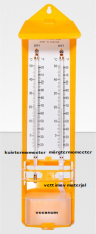
\includegraphics[width=\textwidth,height=0.96\textheight,keepaspectratio=true]{wet-dry-psychrometer} 

}

\caption{Märg-kuiv-psühromeeter ({„Psychrometer Wet \& Dry``} (\protect\hyperlink{ref-psychrometer}{s.a.})).}\label{fig:wet-dry-psychrometer}
\end{figure}

\hypertarget{aspiratsioonpsuxfchromeetriga-uxf5huniiskuse-muxe4uxe4ramine}{%
\subsection{Aspiratsioonpsühromeetriga õhuniiskuse määramine}\label{aspiratsioonpsuxfchromeetriga-uxf5huniiskuse-muxe4uxe4ramine}}

Aspiratsioonpsühromeeter on kujutatud pildil \ref{fig:aspiration-psychrometer}. Aspiratsioonpsühromeeter, nagu nimetuseski, n-ö hingab (\protect\hyperlink{ref-aspirationspsychrometer}{{„Aspirationspsychrometer``} s.a.}).



\begin{Shaded}
\begin{Highlighting}[numbers=left,,]
\FunctionTok{include\_svg}\NormalTok{(}\StringTok{"Aspirations{-}Psychrometer{-}Fotomontage{-}65434{-}LRV1\_3000px\_2048x2048.svg"}\NormalTok{)}
\end{Highlighting}
\end{Shaded}

\begin{figure}

{\centering 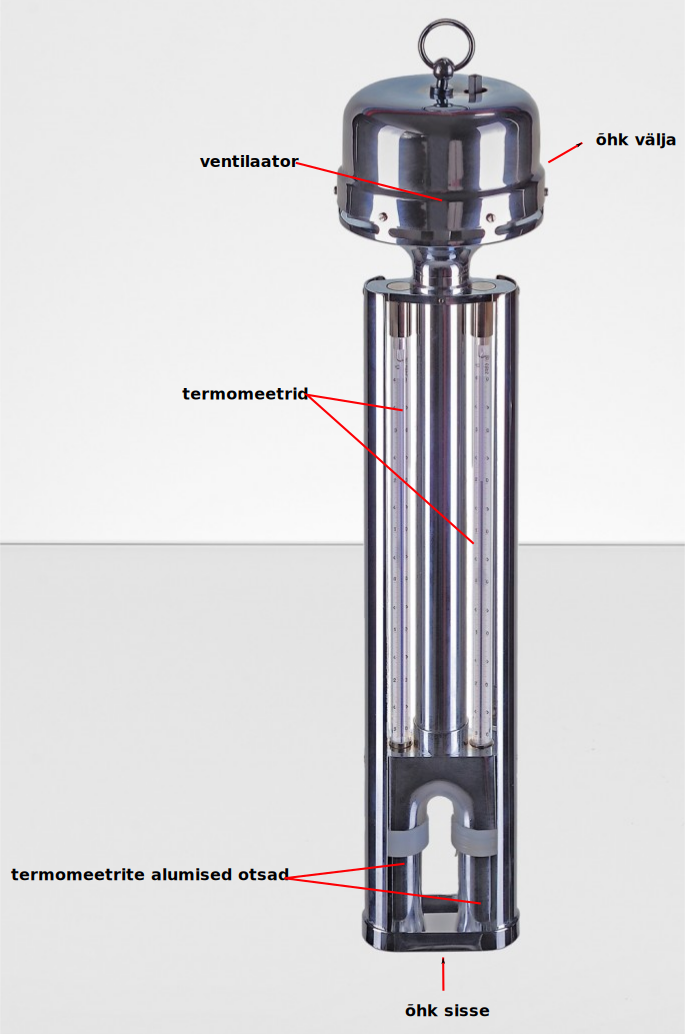
\includegraphics[width=\textwidth,height=0.96\textheight,keepaspectratio=true]{Aspirations-Psychrometer-Fotomontage-65434-LRV1_3000px_2048x2048} 

}

\caption{Aspiratsioonpsühromeeter ({„Aspiration Psychrometer``} (\protect\hyperlink{ref-aspiration}{s.a.})).}\label{fig:aspiration-psychrometer}
\end{figure}

Selles on kaks termomeetrit, millest üks on ühendatud niiskust imava jupiga. Kumb termomeeter ühendada, on vabalt valida. Üks jäetakse kuivtermomeetriks ja teine võetakse märgtermomeetriks. Materjal, mis imab vett, nt riidetükk keritakse ümber ühe termomeetri alumise otsa nagu näidatud pildil \ref{fig:aspiration-psychrometer-installing-batist}.



\begin{Shaded}
\begin{Highlighting}[numbers=left,,]
\FunctionTok{include\_svg}\NormalTok{(}\StringTok{"aspiration{-}psychrometer{-}installing{-}batist.png"}\NormalTok{)}
\end{Highlighting}
\end{Shaded}

\begin{figure}
\includegraphics[width=\textwidth,height=\textheight,keepaspectratio=true]{aspiration-psychrometer-installing-batist} \caption{Aspiratsioonpsühromeetrisse batisti paigaldamine ({„Как пользоваться аспирационным психрометром (ответ зрителю канала).``} (\protect\hyperlink{ref-aspiration_psychrometer_ru}{s.a.})).}\label{fig:aspiration-psychrometer-installing-batist}
\end{figure}

Termomeetri ülaosas on ventilaator, mis tirib õhku läbi mõlema termomeetri toru, mis soodustab aurustumist, mida on vaja niiske otsaga termomeetri jaoks. Kui mõlemast läbi ei tõmbaks, siis oleksid tingimused kummagi termomeetri jaoks erinevad ja me ei saaks näite võrrelda. meie ei kasutanud pildil \ref{fig:aspiration-psychrometer} olevat 2600 eurot maksvat seadet, vaid meil oli kasutuses selline psühromeeter, mis töötab elektri jõul, nii et pole vaja ise lehvitada, puhuda ega keerutada, samuti mitte vedru üles keerata.

Paigaldasime Assmanni aspiratsioonpsühromeetri ühe termomeetri alumise otsa ümber vett imava materjali, mille olime eelnevalt ümbritseva keskkonna temperatuuril oleva destilleeritud veega märjaks teinud, ja lülitasime seadme sisse. Ootasime, kuni niiske otsaga termomeetri näit vähenes. Teoreetiliselt vähenes ka kuivtermomeetri näit, sest õhku tõmmati ka selle otsa juurest läbi. Kui niiske otsaga termomeetri näit enam ei vähenenud, tegime kindlaks kummagi termomeetri näidu ja kandsime tabelisse \ref{tab:data-analysis}.

\hypertarget{uxf5hu-niiskuskarakteristikue-muxe4uxe4ramine-pasco-limasensoriga}{%
\subsection{\texorpdfstring{Õhu niiskuskarakteristikue määramine \emph{Pasco} limasensoriga}{Õhu niiskuskarakteristikue määramine Pasco limasensoriga}}\label{uxf5hu-niiskuskarakteristikue-muxe4uxe4ramine-pasco-limasensoriga}}

\hypertarget{andmeanaluxfcuxfcs}{%
\section{Andmeanalüüs}\label{andmeanaluxfcuxfcs}}

Arvutustes kasutan rõhuna standardset atmosfääri, et tulemused oleksid võrreldavad graafikuga \ref{fig:psychrometric-diagram}.

\begin{Shaded}
\begin{Highlighting}[numbers=left,,]
\NormalTok{method }\OtherTok{\textless{}{-}} \FunctionTok{c}\NormalTok{(}
  \StringTok{"Augusti psühhomeeter"}\NormalTok{,}
  \StringTok{"Assmanni psühhomeeter"}\NormalTok{,}
  \StringTok{"Pasco}
\StringTok{ilmajaama}
\StringTok{andmete järgi}
\StringTok{niiskuse}
\StringTok{karakteristikud"}
\NormalTok{)}

\NormalTok{t\_d }\OtherTok{\textless{}{-}} \FunctionTok{c}\NormalTok{(}\DecValTok{24}\NormalTok{, }\FloatTok{24.6}\NormalTok{, }\FloatTok{26.3}\NormalTok{)}
\FunctionTok{SetUnitSystem}\NormalTok{(}\StringTok{"SI"}\NormalTok{)}
\NormalTok{T\_d }\OtherTok{\textless{}{-}} \FunctionTok{GetTKelvinFromTCelsius}\NormalTok{(t\_d)}
\NormalTok{RH\_Pasco }\OtherTok{\textless{}{-}} \FloatTok{30.8e{-}2}
\NormalTok{t\_w\_Pasco }\OtherTok{\textless{}{-}} \FunctionTok{GetTWetBulbFromRelHum}\NormalTok{(t\_d[}\DecValTok{3}\NormalTok{], RH\_Pasco, p\_at)}
\NormalTok{t\_w }\OtherTok{\textless{}{-}} \FunctionTok{c}\NormalTok{(}\FloatTok{16.5}\NormalTok{, }\FloatTok{15.2}\NormalTok{, t\_w\_Pasco)}
\NormalTok{T\_w }\OtherTok{\textless{}{-}} \FunctionTok{GetTKelvinFromTCelsius}\NormalTok{(t\_w)}
\NormalTok{p\_w\_H2O }\OtherTok{\textless{}{-}} \FunctionTok{calculate\_p\_H2O}\NormalTok{(T\_w)}
\NormalTok{gamma\_w }\OtherTok{\textless{}{-}} \FunctionTok{calculate\_gamma\_H2O}\NormalTok{(p\_w\_H2O, T\_w)}
\NormalTok{p\_dp }\OtherTok{\textless{}{-}} \FunctionTok{calculate\_p\_dp}\NormalTok{(p\_w\_H2O, t\_d, t\_w)}
\NormalTok{gamma\_d }\OtherTok{\textless{}{-}} \FunctionTok{calculate\_gamma\_H2O}\NormalTok{(}\FunctionTok{calculate\_p\_H2O}\NormalTok{(T\_d), T\_d)}
\NormalTok{a }\OtherTok{\textless{}{-}}\NormalTok{ gamma\_w }\SpecialCharTok{*} \FloatTok{1e3} \SpecialCharTok{{-}}\NormalTok{ .}\DecValTok{64} \SpecialCharTok{*}\NormalTok{ (t\_d }\SpecialCharTok{{-}}\NormalTok{ t\_w)}
\NormalTok{p\_d\_H2O }\OtherTok{\textless{}{-}} \FunctionTok{calculate\_p\_H2O}\NormalTok{(T\_d)}
\NormalTok{RH }\OtherTok{\textless{}{-}} \FunctionTok{calculate\_RH}\NormalTok{(p\_dp, p\_d\_H2O)}
\NormalTok{RH\_according\_to\_instructions }\OtherTok{\textless{}{-}}\NormalTok{ a }\SpecialCharTok{/}\NormalTok{ (gamma\_d }\SpecialCharTok{*} \FloatTok{1e3}\NormalTok{) }\SpecialCharTok{*} \DecValTok{100}
\NormalTok{RH\_psychrolib }\OtherTok{\textless{}{-}} \FunctionTok{GetRelHumFromTWetBulb}\NormalTok{(t\_d, t\_w, p\_at)}

\NormalTok{psychrometry }\OtherTok{\textless{}{-}} \FunctionTok{data.frame}\NormalTok{(}
\NormalTok{  method,}
\NormalTok{  t\_d,}
\NormalTok{  T\_d,}
\NormalTok{  gamma\_d,}
\NormalTok{  t\_w,}
\NormalTok{  T\_w,}
\NormalTok{  a,}
\NormalTok{  gamma\_w,}
\NormalTok{  p\_dp,}
\NormalTok{  RH,}
\NormalTok{  RH\_according\_to\_instructions,}
\NormalTok{  RH\_psychrolib}
\NormalTok{)}

\FunctionTok{colnames}\NormalTok{(psychrometry) }\OtherTok{=} \FunctionTok{c}\NormalTok{(}
  \StringTok{"Meetod või sensor"}\NormalTok{,}
  \StringTok{"$}\SpecialCharTok{\textbackslash{}\textbackslash{}}\StringTok{frac\{t\_}\SpecialCharTok{\textbackslash{}\textbackslash{}}\StringTok{text\{d\}\}\{}\SpecialCharTok{\textbackslash{}\textbackslash{}}\StringTok{unit\{}\SpecialCharTok{\textbackslash{}\textbackslash{}}\StringTok{degreeCelsius\}\}$"}\NormalTok{,}
  \StringTok{"$}\SpecialCharTok{\textbackslash{}\textbackslash{}}\StringTok{frac\{T\_}\SpecialCharTok{\textbackslash{}\textbackslash{}}\StringTok{text\{d\}\}\{}\SpecialCharTok{\textbackslash{}\textbackslash{}}\StringTok{unit\{}\SpecialCharTok{\textbackslash{}\textbackslash{}}\StringTok{kelvin\}\}$"}\NormalTok{,}
  \StringTok{"$}\SpecialCharTok{\textbackslash{}\textbackslash{}}\StringTok{frac\{}\SpecialCharTok{\textbackslash{}\textbackslash{}}\StringTok{gamma\_}\SpecialCharTok{\textbackslash{}\textbackslash{}}\StringTok{text\{d\}\}\{}\SpecialCharTok{\textbackslash{}\textbackslash{}}\StringTok{unit\{}\SpecialCharTok{\textbackslash{}\textbackslash{}}\StringTok{kilogram}\SpecialCharTok{\textbackslash{}\textbackslash{}}\StringTok{per}\SpecialCharTok{\textbackslash{}\textbackslash{}}\StringTok{cubic}\SpecialCharTok{\textbackslash{}\textbackslash{}}\StringTok{meter\}\}$"}\NormalTok{,}
  \StringTok{"$}\SpecialCharTok{\textbackslash{}\textbackslash{}}\StringTok{frac\{t\_}\SpecialCharTok{\textbackslash{}\textbackslash{}}\StringTok{text\{w\}\}\{}\SpecialCharTok{\textbackslash{}\textbackslash{}}\StringTok{unit\{}\SpecialCharTok{\textbackslash{}\textbackslash{}}\StringTok{degreeCelsius\}\}$"}\NormalTok{,}
  \StringTok{"$}\SpecialCharTok{\textbackslash{}\textbackslash{}}\StringTok{frac\{T\_}\SpecialCharTok{\textbackslash{}\textbackslash{}}\StringTok{text\{w\}\}\{}\SpecialCharTok{\textbackslash{}\textbackslash{}}\StringTok{unit\{}\SpecialCharTok{\textbackslash{}\textbackslash{}}\StringTok{kelvin\}\}$"}\NormalTok{,}
  \StringTok{"$}\SpecialCharTok{\textbackslash{}\textbackslash{}}\StringTok{frac\{a\}\{}\SpecialCharTok{\textbackslash{}\textbackslash{}}\StringTok{unit\{}\SpecialCharTok{\textbackslash{}\textbackslash{}}\StringTok{gram}\SpecialCharTok{\textbackslash{}\textbackslash{}}\StringTok{per}\SpecialCharTok{\textbackslash{}\textbackslash{}}\StringTok{cubic}\SpecialCharTok{\textbackslash{}\textbackslash{}}\StringTok{meter\} {-} }\SpecialCharTok{\textbackslash{}\textbackslash{}}\StringTok{unit\{}\SpecialCharTok{\textbackslash{}\textbackslash{}}\StringTok{degreeCelsius\}\}$"}\NormalTok{,}
  \StringTok{"$}\SpecialCharTok{\textbackslash{}\textbackslash{}}\StringTok{frac\{}\SpecialCharTok{\textbackslash{}\textbackslash{}}\StringTok{gamma\_}\SpecialCharTok{\textbackslash{}\textbackslash{}}\StringTok{text\{w\}\}\{}\SpecialCharTok{\textbackslash{}\textbackslash{}}\StringTok{unit\{}\SpecialCharTok{\textbackslash{}\textbackslash{}}\StringTok{kilogram}\SpecialCharTok{\textbackslash{}\textbackslash{}}\StringTok{per}\SpecialCharTok{\textbackslash{}\textbackslash{}}\StringTok{cubic}\SpecialCharTok{\textbackslash{}\textbackslash{}}\StringTok{meter\}\}$"}\NormalTok{,}
  \StringTok{"$}\SpecialCharTok{\textbackslash{}\textbackslash{}}\StringTok{frac\{p\_}\SpecialCharTok{\textbackslash{}\textbackslash{}}\StringTok{text\{dp\}(}\SpecialCharTok{\textbackslash{}\textbackslash{}}\StringTok{ce\{H\_2O\})\}\{}\SpecialCharTok{\textbackslash{}\textbackslash{}}\StringTok{unit\{}\SpecialCharTok{\textbackslash{}\textbackslash{}}\StringTok{Pa\}\}$"}\NormalTok{,}
  \StringTok{"$RH$"}\NormalTok{,}
  \StringTok{"Vastavalt juhendile $}\SpecialCharTok{\textbackslash{}\textbackslash{}}\StringTok{frac\{RH\}\{}\SpecialCharTok{\textbackslash{}\textbackslash{}}\StringTok{unit\{}\SpecialCharTok{\textbackslash{}\textbackslash{}}\StringTok{percent\}\}$"}\NormalTok{,}
  \StringTok{"Vastavalt }\SpecialCharTok{\textbackslash{}"}\StringTok{psychrolib}\SpecialCharTok{\textbackslash{}"}\StringTok{ile $RH$"}
\NormalTok{)}


\FunctionTok{print\_table}\NormalTok{(}
\NormalTok{  psychrometry,}
  \AttributeTok{caption =} \StringTok{"Suhtelise niiskuse arvutamise sisend{-} ja väljundandmed, milles $w$ tähendab märga ja $d$ kuiva keskkonda ning $dp$ kastepunkti."}\NormalTok{,}
  \AttributeTok{digits =} \DecValTok{5}
\NormalTok{) }\SpecialCharTok{\%\textgreater{}\%}
  \FunctionTok{column\_spec}\NormalTok{(}\DecValTok{1}\NormalTok{, }\AttributeTok{width =} \StringTok{"6em"}\NormalTok{) }\SpecialCharTok{\%\textgreater{}\%}
  \FunctionTok{column\_spec}\NormalTok{(}\DecValTok{11}\NormalTok{, }\AttributeTok{width =} \StringTok{"5em"}\NormalTok{) }\SpecialCharTok{\%\textgreater{}\%}
  \FunctionTok{column\_spec}\NormalTok{(}\DecValTok{12}\NormalTok{, }\AttributeTok{width =} \StringTok{"5em"}\NormalTok{) }\SpecialCharTok{\%\textgreater{}\%}
  \FunctionTok{landscape}\NormalTok{()}
\end{Highlighting}
\end{Shaded}

\begin{landscape}
\begin{longtable}[t]{>{\raggedright\arraybackslash}p{6em}rrrrrrrrr>{\raggedleft\arraybackslash}p{5em}>{\raggedleft\arraybackslash}p{5em}}
\caption{\label{tab:data-analysis}Suhtelise niiskuse arvutamise sisend- ja väljundandmed, milles $w$ tähendab märga ja $d$ kuiva keskkonda ning $dp$ kastepunkti.}\\
\toprule
\multicolumn{1}{c}{} \\

Meetod või sensor & $\frac{t_\text{d}}{\unit{\degreeCelsius}}$ & $\frac{T_\text{d}}{\unit{\kelvin}}$ & $\frac{\gamma_\text{d}}{\unit{\kilogram\per\cubic\meter}}$ & $\frac{t_\text{w}}{\unit{\degreeCelsius}}$ & $\frac{T_\text{w}}{\unit{\kelvin}}$ & $\frac{a}{\unit{\gram\per\cubic\meter} - \unit{\degreeCelsius}}$ & $\frac{\gamma_\text{w}}{\unit{\kilogram\per\cubic\meter}}$ & $\frac{p_\text{dp}(\ce{H_2O})}{\unit{\Pa}}$ & $RH$ & Vastavalt juhendile $\frac{RH}{\unit{\percent}}$ & Vastavalt "psychrolib"ile $RH$\\
\midrule
\endfirsthead
\caption[]{Suhtelise niiskuse arvutamise sisend- ja väljundandmed, milles $w$ tähendab märga ja $d$ kuiva keskkonda ning $dp$ kastepunkti. $\textit{(Jätkub...)}$}\\
\toprule
\multicolumn{1}{c}{} \\

Meetod või sensor & $\frac{t_\text{d}}{\unit{\degreeCelsius}}$ & $\frac{T_\text{d}}{\unit{\kelvin}}$ & $\frac{\gamma_\text{d}}{\unit{\kilogram\per\cubic\meter}}$ & $\frac{t_\text{w}}{\unit{\degreeCelsius}}$ & $\frac{T_\text{w}}{\unit{\kelvin}}$ & $\frac{a}{\unit{\gram\per\cubic\meter} - \unit{\degreeCelsius}}$ & $\frac{\gamma_\text{w}}{\unit{\kilogram\per\cubic\meter}}$ & $\frac{p_\text{dp}(\ce{H_2O})}{\unit{\Pa}}$ & $RH$ & Vastavalt juhendile $\frac{RH}{\unit{\percent}}$ & Vastavalt "psychrolib"ile $RH$\\
\midrule
\endhead
\midrule
\multicolumn{12}{r@{}}{Tabel järgneb järgmisel leheküljel...}\
\endfoot
\bottomrule
\endlastfoot
\cellcolor{gray!6}{Augusti psühhomeeter} & \cellcolor{gray!6}{24.0} & \cellcolor{gray!6}{297.15} & \cellcolor{gray!6}{0.02177} & \cellcolor{gray!6}{16.50000} & \cellcolor{gray!6}{289.6500} & \cellcolor{gray!6}{9.24372} & \cellcolor{gray!6}{0.01404} & \cellcolor{gray!6}{1374.090} & \cellcolor{gray!6}{0.46031} & \cellcolor{gray!6}{42.46700} & \cellcolor{gray!6}{0.46446}\\
Assmanni psühhomeeter & 24.6 & 297.75 & 0.02252 & 15.20000 & 288.3500 & 6.96524 & 0.01298 & 1096.775 & 0.35444 & 30.93141 & 0.35947\\
Pasco
ilmajaama
andmete järgi
niiskuse
\cellcolor{gray!6}{karakteristikud} & \cellcolor{gray!6}{26.3} & \cellcolor{gray!6}{299.45} & \cellcolor{gray!6}{0.02477} & \cellcolor{gray!6}{15.49968} & \cellcolor{gray!6}{288.6497} & \cellcolor{gray!6}{6.30757} & \cellcolor{gray!6}{0.01322} & \cellcolor{gray!6}{1036.382} & \cellcolor{gray!6}{0.30274} & \cellcolor{gray!6}{25.46449} & \cellcolor{gray!6}{0.30800}\\*
\end{longtable}
\end{landscape}

\textbackslash end\{landscape\}

\begin{Shaded}
\begin{Highlighting}[numbers=left,,]

\NormalTok{librarian}\SpecialCharTok{::}\FunctionTok{shelf}\NormalTok{(}\StringTok{"psychrolib"}\NormalTok{)}
\CommentTok{\# psychometrics \textless{}{-} CalcPsychrometricsFromTWetBulb(t, t1, p\_at)}
\CommentTok{\# print(psychometrics)}
\CommentTok{\# GetDegreeOfSaturation(t, psychometrics$HumRatio, p\_at)}
\FunctionTok{GetDryAirVolume}\NormalTok{(t, p\_at)}
\CommentTok{\#\textgreater{}   [1] 0.7738023 0.7794681 0.7851339 0.7907996 0.7964654 0.8021312 0.8077970}
\CommentTok{\#\textgreater{}   [8] 0.8134627 0.8162956 0.8165789 0.8168622 0.8171455 0.8174288 0.8177120}
\CommentTok{\#\textgreater{}  [15] 0.8179953 0.8182786 0.8185619 0.8188452 0.8191285 0.8194118 0.8196951}
\CommentTok{\#\textgreater{}  [22] 0.8199784 0.8202616 0.8205449 0.8208282 0.8211115 0.8213948 0.8216781}
\CommentTok{\#\textgreater{}  [29] 0.8219614 0.8222447 0.8225280 0.8228112 0.8230945 0.8233778 0.8236611}
\CommentTok{\#\textgreater{}  [36] 0.8239444 0.8242277 0.8245110 0.8247943 0.8250775 0.8253608 0.8256441}
\CommentTok{\#\textgreater{}  [43] 0.8259274 0.8262107 0.8264940 0.8267773 0.8270606 0.8273439 0.8276271}
\CommentTok{\#\textgreater{}  [50] 0.8279104 0.8281937 0.8284770 0.8287603 0.8290436 0.8293269 0.8296102}
\CommentTok{\#\textgreater{}  [57] 0.8298935 0.8301767 0.8304600 0.8307433 0.8310266 0.8313099 0.8315932}
\CommentTok{\#\textgreater{}  [64] 0.8318765 0.8321598 0.8324430 0.8327263 0.8330096 0.8332929 0.8335762}
\CommentTok{\#\textgreater{}  [71] 0.8338595 0.8341428 0.8344261 0.8347094 0.8349926 0.8352759 0.8355592}
\CommentTok{\#\textgreater{}  [78] 0.8358425 0.8361258 0.8364091 0.8366924 0.8369757 0.8372589 0.8375422}
\CommentTok{\#\textgreater{}  [85] 0.8378255 0.8381088 0.8383921 0.8386754 0.8389587 0.8392420 0.8395253}
\CommentTok{\#\textgreater{}  [92] 0.8398085 0.8400918 0.8403751 0.8406584 0.8409417 0.8412250 0.8415083}
\CommentTok{\#\textgreater{}  [99] 0.8417916 0.8420749 0.8423581 0.8426414 0.8429247 0.8432080 0.8434913}
\CommentTok{\#\textgreater{} [106] 0.8437746 0.8440579 0.8443412 0.8446244 0.8449077 0.8451910 0.8454743}
\CommentTok{\#\textgreater{} [113] 0.8457576 0.8460409 0.8463242 0.8466075 0.8468908 0.8471740 0.8474573}
\CommentTok{\#\textgreater{} [120] 0.8477406 0.8480239 0.8483072 0.8485905 0.8488738 0.8491571 0.8494404}
\CommentTok{\#\textgreater{} [127] 0.8497236 0.8500069 0.8502902 0.8505735 0.8508568 0.8511401 0.8514234}
\CommentTok{\#\textgreater{} [134] 0.8517067 0.8519899 0.8522732 0.8525565 0.8528398 0.8531231 0.8644546}
\CommentTok{\#\textgreater{} [141] 0.8757862 0.8871177 0.8984493 0.9097808 0.9211123 0.9324439 0.9437754}
\CommentTok{\#\textgreater{} [148] 0.9551069 0.9664385 0.9777700 0.9891015 1.0004331 1.0117646 1.0230962}
\CommentTok{\#\textgreater{} [155] 1.0344277 1.0457592 1.0570908 1.0684223 1.0797538 1.0910854 1.1024169}
\CommentTok{\#\textgreater{} [162] 1.1137485 1.1250800 1.1364115 1.1477431 1.1590746 1.1704061 1.1817377}
\CommentTok{\#\textgreater{} [169] 1.1930692 1.2044008 1.2157323 1.2270638 1.2383954 1.2497269 1.2610584}
\CommentTok{\#\textgreater{} [176] 1.2723900 1.2837215 1.2950531 1.3063846 1.3177161 1.3290477 1.3403792}
\CommentTok{\# GetMoistAirDensity(t, psychometrics$HumRatio, p\_at)}
\CommentTok{\# GetMoistAirVolume(t, psychometrics$HumRatio, p\_at)}
\FunctionTok{GetSatVapPres}\NormalTok{(t)}
\CommentTok{\#\textgreater{}   [1]     611.1536     705.9544     813.4799     935.2456    1072.8405}
\CommentTok{\#\textgreater{}   [6]    1227.9953    1402.5912    1598.6692    1705.4478    1716.4624}
\CommentTok{\#\textgreater{}  [11]    1727.5395    1738.6793    1749.8821    1761.1483    1772.4781}
\CommentTok{\#\textgreater{}  [16]    1783.8718    1795.3297    1806.8522    1818.4396    1830.0921}
\CommentTok{\#\textgreater{}  [21]    1841.8101    1853.5938    1865.4437    1877.3600    1889.3430}
\CommentTok{\#\textgreater{}  [26]    1901.3931    1913.5105    1925.6957    1937.9488    1950.2702}
\CommentTok{\#\textgreater{}  [31]    1962.6603    1975.1194    1987.6478    2000.2458    2012.9137}
\CommentTok{\#\textgreater{}  [36]    2025.6520    2038.4608    2051.3406    2064.2916    2077.3143}
\CommentTok{\#\textgreater{}  [41]    2090.4089    2103.5758    2116.8153    2130.1278    2143.5135}
\CommentTok{\#\textgreater{}  [46]    2156.9729    2170.5063    2184.1140    2197.7964    2211.5538}
\CommentTok{\#\textgreater{}  [51]    2225.3865    2239.2950    2253.2795    2267.3404    2281.4781}
\CommentTok{\#\textgreater{}  [56]    2295.6929    2309.9852    2324.3554    2338.8037    2353.3306}
\CommentTok{\#\textgreater{}  [61]    2367.9364    2382.6214    2397.3861    2412.2308    2427.1559}
\CommentTok{\#\textgreater{}  [66]    2442.1616    2457.2485    2472.4169    2487.6671    2502.9995}
\CommentTok{\#\textgreater{}  [71]    2518.4145    2533.9125    2549.4938    2565.1589    2580.9080}
\CommentTok{\#\textgreater{}  [76]    2596.7416    2612.6601    2628.6638    2644.7532    2660.9286}
\CommentTok{\#\textgreater{}  [81]    2677.1903    2693.5389    2709.9746    2726.4979    2743.1092}
\CommentTok{\#\textgreater{}  [86]    2759.8089    2776.5973    2793.4748    2810.4419    2827.4990}
\CommentTok{\#\textgreater{}  [91]    2844.6464    2861.8846    2879.2139    2896.6348    2914.1477}
\CommentTok{\#\textgreater{}  [96]    2931.7529    2949.4510    2967.2422    2985.1271    3003.1060}
\CommentTok{\#\textgreater{} [101]    3021.1793    3039.3475    3057.6110    3075.9702    3094.4255}
\CommentTok{\#\textgreater{} [106]    3112.9774    3131.6262    3150.3724    3169.2165    3188.1588}
\CommentTok{\#\textgreater{} [111]    3207.1998    3226.3399    3245.5795    3264.9192    3284.3592}
\CommentTok{\#\textgreater{} [116]    3303.9001    3323.5423    3343.2863    3363.1324    3383.0811}
\CommentTok{\#\textgreater{} [121]    3403.1329    3423.2883    3443.5476    3463.9113    3484.3798}
\CommentTok{\#\textgreater{} [126]    3504.9537    3525.6334    3546.4193    3567.3118    3588.3116}
\CommentTok{\#\textgreater{} [131]    3609.4189    3630.6343    3651.9582    3673.3911    3694.9335}
\CommentTok{\#\textgreater{} [136]    3716.5858    3738.3485    3760.2220    3782.2070    4758.5342}
\CommentTok{\#\textgreater{} [141]    5946.6419    7383.4600    9110.6747   11175.0879   13628.9751}
\CommentTok{\#\textgreater{} [146]   16530.4400   19943.7606   23939.7270   28595.9672   33997.2585}
\CommentTok{\#\textgreater{} [151]   40235.8242   47411.6115   55632.5514   65014.7983   75682.9489}
\CommentTok{\#\textgreater{} [156]   87770.2384  101418.7168  116779.4013  134012.4076  153287.0601}
\CommentTok{\#\textgreater{} [161]  174781.9806  198685.1571  225193.9935  254515.3412  286865.5139}
\CommentTok{\#\textgreater{} [166]  322470.2868  361564.8822  404393.9412  451211.4861  502280.8714}
\CommentTok{\#\textgreater{} [171]  557874.7278  618274.8994  683772.3751  754667.2172  831268.4868}
\CommentTok{\#\textgreater{} [176]  913894.1683 1002871.0943 1098534.8710 1201229.8062 1311308.8405}
\CommentTok{\#\textgreater{} [181] 1429133.4820 1555073.7456}
\FunctionTok{GetStandardAtmPressure}\NormalTok{(}\DecValTok{10}\NormalTok{)}
\CommentTok{\#\textgreater{} [1] 101204.9}
\FunctionTok{GetStationPressure}\NormalTok{(p\_at, }\DecValTok{10}\NormalTok{, t)}
\CommentTok{\#\textgreater{}   [1] 101198.4 101199.3 101200.2 101201.1 101202.0 101202.8 101203.7 101204.5}
\CommentTok{\#\textgreater{}   [9] 101204.9 101205.0 101205.0 101205.1 101205.1 101205.2 101205.2 101205.2}
\CommentTok{\#\textgreater{}  [17] 101205.3 101205.3 101205.4 101205.4 101205.4 101205.5 101205.5 101205.6}
\CommentTok{\#\textgreater{}  [25] 101205.6 101205.7 101205.7 101205.7 101205.8 101205.8 101205.9 101205.9}
\CommentTok{\#\textgreater{}  [33] 101205.9 101206.0 101206.0 101206.1 101206.1 101206.1 101206.2 101206.2}
\CommentTok{\#\textgreater{}  [41] 101206.3 101206.3 101206.3 101206.4 101206.4 101206.5 101206.5 101206.6}
\CommentTok{\#\textgreater{}  [49] 101206.6 101206.6 101206.7 101206.7 101206.8 101206.8 101206.8 101206.9}
\CommentTok{\#\textgreater{}  [57] 101206.9 101207.0 101207.0 101207.0 101207.1 101207.1 101207.2 101207.2}
\CommentTok{\#\textgreater{}  [65] 101207.2 101207.3 101207.3 101207.4 101207.4 101207.4 101207.5 101207.5}
\CommentTok{\#\textgreater{}  [73] 101207.6 101207.6 101207.6 101207.7 101207.7 101207.8 101207.8 101207.8}
\CommentTok{\#\textgreater{}  [81] 101207.9 101207.9 101208.0 101208.0 101208.0 101208.1 101208.1 101208.2}
\CommentTok{\#\textgreater{}  [89] 101208.2 101208.2 101208.3 101208.3 101208.3 101208.4 101208.4 101208.5}
\CommentTok{\#\textgreater{}  [97] 101208.5 101208.5 101208.6 101208.6 101208.7 101208.7 101208.7 101208.8}
\CommentTok{\#\textgreater{} [105] 101208.8 101208.9 101208.9 101208.9 101209.0 101209.0 101209.1 101209.1}
\CommentTok{\#\textgreater{} [113] 101209.1 101209.2 101209.2 101209.2 101209.3 101209.3 101209.4 101209.4}
\CommentTok{\#\textgreater{} [121] 101209.4 101209.5 101209.5 101209.6 101209.6 101209.6 101209.7 101209.7}
\CommentTok{\#\textgreater{} [129] 101209.7 101209.8 101209.8 101209.9 101209.9 101209.9 101210.0 101210.0}
\CommentTok{\#\textgreater{} [137] 101210.1 101210.1 101210.1 101211.6 101213.1 101214.5 101215.9 101217.3}
\CommentTok{\#\textgreater{} [145] 101218.6 101219.9 101221.2 101222.4 101223.6 101224.8 101225.9 101227.0}
\CommentTok{\#\textgreater{} [153] 101228.1 101229.2 101230.3 101231.3 101232.3 101233.3 101234.2 101235.2}
\CommentTok{\#\textgreater{} [161] 101236.1 101237.0 101237.9 101238.7 101239.6 101240.4 101241.3 101242.1}
\CommentTok{\#\textgreater{} [169] 101242.8 101243.6 101244.4 101245.1 101245.8 101246.6 101247.3 101248.0}
\CommentTok{\#\textgreater{} [177] 101248.6 101249.3 101250.0 101250.6 101251.2 101251.9}
\CommentTok{\# GetVaporPressureDeficit(t, psychometrics$HumRatio, p\_at)}
\CommentTok{\# GetVapPresFromHumRatio(psychometrics$HumRatio, p\_at)}
\CommentTok{\# \textgreater{} 1/69.006*1000{-}.64*(24{-}16.5)}
\CommentTok{\# [1] 9.691493}
\CommentTok{\# \textgreater{} 9.691493/(1/45.863*1000)}
\CommentTok{\# [1] 0.4444809}
\CommentTok{\# \textgreater{} .5/755*1013.25}
\CommentTok{\# [1] 0.6710265}
\NormalTok{librarian}\SpecialCharTok{::}\FunctionTok{shelf}\NormalTok{(}\StringTok{"MeTo"}\NormalTok{)}
\FunctionTok{psyc\_cons}\NormalTok{(}\AttributeTok{elev =} \DecValTok{2}\NormalTok{, }\AttributeTok{P =} \FloatTok{101.3}\NormalTok{)}
\CommentTok{\#\textgreater{} [1] 0.06733834}
\CommentTok{\# \textgreater{} {-}5.8002206e3/(24+273.15) + 1.3914993e0 {-} 4.8640239e{-}2*(24+273.15) + 4.1764768e{-}5*(24+273.15)\^{}2 {-} 1.4452093e{-}8*(24+273.15)\^{}3 + 6.5459673e0*log((24+273.15))}
\CommentTok{\# [1] 8.001398}
\CommentTok{\# \textgreater{} exp(1)\^{}8.001398}
\CommentTok{\# [1] 2985.128}
\CommentTok{\# \textgreater{} 2985.128*.018/8.314472/(24+273.15)}
\CommentTok{\# [1] 0.02174829}
\end{Highlighting}
\end{Shaded}

\begin{Shaded}
\begin{Highlighting}[numbers=left,,]
\NormalTok{t\_dp\_Pasco }\OtherTok{\textless{}{-}} \FloatTok{6.8}
\NormalTok{T\_dp\_Pasco }\OtherTok{\textless{}{-}} \FunctionTok{GetTKelvinFromTCelsius}\NormalTok{(t\_dp\_Pasco)}
\NormalTok{p\_dp }\OtherTok{\textless{}{-}} \FunctionTok{calculate\_p\_H2O}\NormalTok{(T\_dp\_Pasco)}
\NormalTok{p\_d }\OtherTok{\textless{}{-}} \FunctionTok{calculate\_p\_H2O}\NormalTok{(}\FunctionTok{GetTKelvinFromTCelsius}\NormalTok{(t\_d[}\DecValTok{3}\NormalTok{]))}
\NormalTok{RH }\OtherTok{\textless{}{-}} \FunctionTok{calculate\_RH}\NormalTok{(p\_dp, p\_d)}
\NormalTok{t\_dp\_r }\OtherTok{\textless{}{-}} \FloatTok{5.9}
\NormalTok{T\_dp\_r }\OtherTok{\textless{}{-}} \FunctionTok{GetTKelvinFromTCelsius}\NormalTok{(t\_dp\_r)}
\end{Highlighting}
\end{Shaded}

Pasco ilmajaamaga väljamõõdetud kastepunkt oli \(\qty{6.8}{\degreeCelsius}\) ehk \(\qty{279.95}{\kelvin}\). Selle kaudu arvutatud õhuniiskus oli 0.2886962.

Katseliselt mõõtsime kastepunktiks \(\qty{5.9}{\degreeCelsius}\) ehk \(\qty{279.05}{\kelvin}\).

\onecolumn

\hypertarget{kasutatud-allikad}{%
\section*{Kasutatud allikad}\label{kasutatud-allikad}}
\addcontentsline{toc}{section}{Kasutatud allikad}

\hyphenpenalty=10000

\markboth{References}{References}

\noindent

\setlength{\parindent}{-0.20in}

\hypertarget{refs}{}
\begin{CSLReferences}{1}{0}
\leavevmode\vadjust pre{\hypertarget{ref-American_Society_of_Heating_Refrigerating_and_Air-Conditioning_Engineers2017-im}{}}%
American Society of Heating, Refrigerating and Air-Conditioning Engineers. 2017. \emph{{ASHRAE} handbook an instrument of service prepared for the profession ; containing a techn. data sect. of reference material}. New York NY: American Soc. of Heating Refrigerating; Air-Conditioning Engineers.

\leavevmode\vadjust pre{\hypertarget{ref-aspiration}{}}%
{„Aspiration Psychrometer``}. s.a. Cassens \& Plath. Vaadatud 25. juuni 2022. \url{https://shop.cassens-plath.de/en/detail/index/sArticle/231}.

\leavevmode\vadjust pre{\hypertarget{ref-aspirationspsychrometer}{}}%
{„Aspirationspsychrometer``}. s.a. www.youtube.com. Vaadatud 25. juuni 2022. \url{https://youtu.be/xFVgA3E6DKE}.

\leavevmode\vadjust pre{\hypertarget{ref-a2018_determination}{}}%
{„Determination of Humidity -- Psychometric Method``}. 2018. Labmonk. \url{https://labmonk.com/determination-of-humidity-psychometric-method}.

\leavevmode\vadjust pre{\hypertarget{ref-RN23688432420080101}{}}%
Gatley, D. P., S. Herrmann, ja H.-J. Kretzschmar. 2008. {„A Twenty-First Century Molar Mass for Dry Air.``} \emph{INTERNATIONAL JOURNAL OF HEATING VENTILATION AIR CONDITIONING AND REFRIGERATING RESEARCH} 14 (5): 655--62. \url{http://ezproxy.tlu.ee/login?url=https://search.ebscohost.com/login.aspx?direct=true\&db=edsbl\&AN=RN236884324\&site=eds-live}.

\leavevmode\vadjust pre{\hypertarget{ref-haynes_2014_crc}{}}%
Haynes, William M. 2014. \emph{CRC Handbook of Chemistry and Physics, 95th Edition}. Taylor \& Francis Ltd.

\leavevmode\vadjust pre{\hypertarget{ref-news_september}{}}%
News, Ocean. s.a. {„September - Moisture Control In Subsea Housings \textbar{} Featured Stories``}. ONT. \url{https://www.oceannews.com/featured-stories/september-moisture-control-in-subsea-housings}.

\leavevmode\vadjust pre{\hypertarget{ref-NOAA_GML_CCGG_Group2019-oq}{}}%
NOAA GML CCGG Group. 2019. {„{NOAA} global monitoring laboratory carbon cycle and greenhouse gases group continuous insitu measurements of {CO2} at global background sites, 1973-present``}. NOAA GML CCGG Group.

\leavevmode\vadjust pre{\hypertarget{ref-psychrometer}{}}%
{„Psychrometer Wet \& Dry``}. s.a. Cassens \& Plath. Vaadatud 25. juuni 2022. \url{https://shop.cassens-plath.de/en/nautical-inventory/weather-measuring-devices/230/psychrometer-wet-dry?c=52\#P:2}.

\leavevmode\vadjust pre{\hypertarget{ref-psychrometric-chart}{}}%
{„PSYCHROMETRIC CHART - US and SI Units``}. s.a. Workforce Development Online for the HVACR Industry.

\leavevmode\vadjust pre{\hypertarget{ref-Whipple_1933}{}}%
Whipple, F J W. 1933. {„The wet-and-dry-bulb hygrometer: the relation to theory of the experimental researches of Awbery and Griffiths``}. \emph{Proceedings of the Physical Society} 45 (2): 307--19. \url{https://doi.org/10.1088/0959-5309/45/2/314}.

\leavevmode\vadjust pre{\hypertarget{ref-aspiration_psychrometer_ru}{}}%
{„Как пользоваться аспирационным психрометром (ответ зрителю канала).``} s.a. www.youtube.com. Vaadatud 25. juuni 2022. \url{https://youtu.be/0WHbF85WSpk}.

\end{CSLReferences}

\end{document}
